\documentclass[12pt,a4paper]{article}

% ============================================
% PACKAGES
% ============================================
\usepackage[utf8]{inputenc}
\usepackage[T1]{fontenc}
\usepackage{amsmath,amssymb,amsfonts}
\usepackage{mathtools}
\usepackage{booktabs}
\usepackage{longtable}
\usepackage{array}
\usepackage{multirow}
\usepackage{graphicx}
\usepackage{float}
\usepackage{caption}
\usepackage{subcaption}
\usepackage{geometry}
\usepackage{setspace}
\usepackage{parskip}
\usepackage{enumitem}
\usepackage{xcolor}
\usepackage{hyperref}
\usepackage{cleveref}
\usepackage{fancyhdr}
\usepackage{titlesec}
\usepackage{tocloft}
\usepackage{pgfplots}
\usepackage{tikz}
\pgfplotsset{compat=1.18}
\usetikzlibrary{patterns,calc,shapes.geometric,arrows.meta,positioning}
\usepackage{pgf-pie}

% ============================================
% TABLE OF CONTENTS FORMATTING
% ============================================
\setlength{\cftsecnumwidth}{3em}
\setlength{\cftsubsecnumwidth}{3.5em}
\setlength{\cftsubsubsecnumwidth}{4.5em}

% ============================================
% PAGE LAYOUT
% ============================================
\geometry{
    left=1.5in,
    right=1in,
    top=1in,
    bottom=1in
}

% ============================================
% LINE SPACING
% ============================================
\onehalfspacing

% ============================================
% HEADER AND FOOTER
% ============================================
\pagestyle{fancy}
\fancyhf{}
\fancyhead[R]{\thepage}
\fancyhead[L]{\nouppercase{\leftmark}}
\renewcommand{\headrulewidth}{0.4pt}

% ============================================
% SECTION FORMATTING
% ============================================
\titleformat{\section}
    {\normalfont\Large\bfseries}{\thesection}{1em}{}
\titleformat{\subsection}
    {\normalfont\large\bfseries}{\thesubsection}{1em}{}
\titleformat{\subsubsection}
    {\normalfont\normalsize\bfseries}{\thesubsubsection}{1em}{}

% ============================================
% HYPERREF SETUP
% ============================================
\hypersetup{
    colorlinks=true,
    linkcolor=blue,
    filecolor=magenta,
    urlcolor=cyan,
    citecolor=blue,
    pdftitle={Frontier-Based Optimization Analysis of Pension Fund Efficiency in Zimbabwe Using Data Envelopment Analysis},
    pdfauthor={Lorraine Mujuru},
    bookmarks=true,
}

% ============================================
% DOCUMENT BEGIN
% ============================================
\begin{document}

% ============================================
% COVER PAGE
% ============================================
\thispagestyle{empty}
\begin{center}


\includegraphics[width=0.5\textwidth]{hit_logo.png}

\vspace{0.3cm}

{\normalsize\bfseries SCHOOL OF BUSINESS AND MANAGEMENT SCIENCES}\\[0.2cm]
{\normalsize\bfseries DEPARTMENT OF FINANCIAL ENGINEERING}

\vspace{1.5cm}

{\large\bfseries FRONTIER -- BASED OPTIMIZATION ANALYSIS OF PENSION FUND EFFICIENCY IN ZIMBABWE USING DATA ENVELOPMENT ANALYSIS (DEA)}

\vspace{1.5cm}

{\normalsize BY}

\vspace{0.5cm}

{\large\bfseries LORRAINE MUJURU}\\[0.2cm]
{\large\bfseries H220021Y}

\vspace{1cm}

{\small THIS RESEARCH IS SUBMITTED TO THE DEPARTMENT OF FINANCIAL ENGINEERING SCHOOL OF BUSINESS AND MANAGEMENT SCIENCES IN PARTIAL FULFILMENT OF THE BACHELOR OF TECHNOLOGY HONOURS DEGREE IN FINANCIAL ENGINEERING}

\vspace{1cm}

{\large\bfseries 2026}

\end{center}

\newpage

% ============================================
% TABLE OF CONTENTS
% ============================================
\tableofcontents
\newpage

% ============================================
% CHAPTER 1: INTRODUCTION
% ============================================
\begin{center}
    {\LARGE\bfseries CHAPTER 1}\\[0.5cm]
    {\Large\bfseries Introduction}
\end{center}
\setcounter{section}{0}
\renewcommand{\thesection}{1.\arabic{section}}
\phantomsection
\addcontentsline{toc}{section}{\textbf{CHAPTER 1: INTRODUCTION}}

\vspace{1cm}

% ============================================
% 1.1 BACKGROUND TO THE STUDY
% ============================================
\section{Background to the Study}

A pension fund is a massive pool of capital specifically designed to provide people with an income after they stop working. These pension funds are among the most significant long-term institutional investors in modern financial systems, responsible for mobilizing savings and allocating capital across financial markets in support of retirement income security and economic development (OECD, 2022). By pooling contributions and investing on behalf of members, pension funds influence capital formation, financial market stability, and intergenerational welfare (World Bank, 2019). As key components of any social protection architecture, retirement arrangements work alongside state systems of support, and individual savings in order to provide an additional or primary income stream and provide financial security to those who are older or no longer in employment (World Bank, 2020). With the reality of demographic aging and changes in labour markets, pension funds have also increasingly been acting as guardians of longer-term savings, major institutional investors, and important providers of stability in national financial systems (OECD, 2022). The ability of funds to function with efficiency, build trust and ensure their members can access their rightful pensions in a timely and reliable manner is very much dependent on their operational effectiveness and successful management (Barr \& Diamond, 2016).

\subsection{Historical Development of Pension Funds}

The origins of organised pension provision can be traced to the late nineteenth century, when Otto von Bismarck introduced Germany's Old Age and Disability Insurance Law in 1889 --- widely regarded as the first state-sponsored pension system in the world (World Bank, 1994). This foundational development established the principle of mandatory, contribution-linked retirement income and inspired similar reforms across Europe and North America during the early twentieth century. In the United States, the Social Security Act of 1935 formalised public pension provision as a response to the mass unemployment and elderly poverty of the Great Depression. The post-Second World War decades saw a rapid proliferation of occupational pension schemes as employers sought to attract and retain workers through deferred compensation arrangements, giving rise to the defined benefit (DB) model that dominated private-sector pension provision for much of the twentieth century (Barr and Diamond, 2016).

From the 1980s onwards, a structural shift occurred in pension fund design as the fiscal unsustainability of defined benefit obligations became apparent in the context of population ageing and rising life expectancy. Defined contribution (DC) schemes, in which members bear investment risk directly, gained ascendancy across developed economies --- particularly following the United States Employee Retirement Income Security Act (ERISA) of 1974 and the subsequent growth of 401(k)-type arrangements. By the early 2000s, multi-pillar pension architectures --- combining mandatory public, mandatory private, and voluntary private pillars --- had been adopted or recommended across a wide range of economies (World Bank, 1994; OECD, 2021). This diversification of pension structure intensified the importance of performance and efficiency measurement, as fund assets under management grew to represent a significant proportion of national financial wealth.

\subsection{Pension Fund Development in Zimbabwe}

Zimbabwe's pension fund sector has a history dating to the colonial era, when occupational pension schemes were established primarily to serve the white-collar workforce within parastatal and mining organisations. Following independence in 1980, successive governments expanded the regulatory framework for pension provision, and the Insurance and Pensions Commission (IPEC) was established under the Insurance Act to provide regulatory oversight of both the insurance and pension industries (IPEC, 2023). The sector grew to encompass a range of self-administered standalone funds, insured funds managed by insurance companies, and occupational provident funds across both public and private sectors.

Zimbabwe's pension fund sector has, however, been severely disrupted by macroeconomic instability. The hyperinflationary crisis of 2007--2008, during which Zimbabwe recorded the highest peacetime inflation rate ever measured, effectively wiped out the real value of pension savings accumulated over decades. The subsequent adoption of a multi-currency regime in 2009 and the eventual re-introduction of a domestic currency under successive currency reform programmes created persistent challenges for fund valuation, asset pricing, and benefit adequacy. These structural disruptions rendered the Zimbabwean pension fund sector particularly vulnerable to managerial inefficiency, as funds struggled to preserve real asset values in an environment of currency volatility, illiquid capital markets, and constrained investment opportunities (IPEC, 2023). Against this backdrop, the operational efficiency of pension fund management assumes heightened significance: inefficient resource utilisation not only erodes returns for members but directly threatens the financial sustainability of the pension system itself.

\subsection{Efficiency Measurement in Financial Institutions}

In evaluating pension fund performance, traditional indicators such as nominal returns, funding ratios, and solvency measures have been widely applied. However, these indicators provide limited insight into how efficiently pension funds utilize their available financial and operational resources (Eling and Luhnen, 2010). As a result, frontier-based efficiency measurement techniques have gained prominence in the financial economics and operations research literature. The seminal contribution of Farrell (1957) introduced the concept of technical efficiency as the ability of a production unit to maximise output from a given set of inputs, and laid the groundwork for the development of non-parametric efficiency frontier methods. Building on Farrell's framework, Charnes, Cooper and Rhodes (1978) developed Data Envelopment Analysis (DEA) --- a linear programming-based technique that constructs an empirical efficiency frontier from observed data without imposing a parametric functional form on the production technology.

Data Envelopment Analysis (DEA) is a non-parametric optimization technique that has been extensively applied to evaluate the relative efficiency of financial institutions, including banks, insurance companies, and pension funds (Charnes, Cooper and Rhodes, 1978; Cooper, Seiford and Tone, 2013). DEA allows for the assessment of efficiency without imposing restrictive assumptions on the production technology, making it particularly suitable for financial institutions with complex input--output relationships. Subsequent extensions of the DEA framework, notably the BCC model introduced by Banker, Charnes and Cooper (1984), allowed for the decomposition of technical efficiency into pure technical efficiency and scale efficiency, enabling researchers to distinguish between inefficiencies arising from managerial decisions and those attributable to sub-optimal scale of operation. These methodological advancements have been widely applied to evaluate efficiency in banking, insurance, and pension fund management across both developed and emerging economies (Kaffash et al., 2020; Barros and Garcia, 2006).

Despite the growing international literature on pension fund efficiency, empirical evidence from developing economies remains limited. This gap is especially pronounced in Zimbabwe, where pension funds operate under conditions of macroeconomic volatility, high inflation, currency instability, and constrained capital markets (OECD, 2021). These conditions have historically affected asset values, investment strategies, and the real purchasing power of retirement benefits.

Given the unique institutional and economic environment in Zimbabwe, there is a need for a rigorous, quantitative assessment of pension fund efficiency that goes beyond descriptive performance measures. This study responds to that need by applying a DEA-based efficiency framework tailored to the Zimbabwean pension fund sector.

% ============================================
% 1.2 STATEMENT OF THE PROBLEM
% ============================================
\section{Statement of the Problem}

Although pension funds play a critical role in Zimbabwe's financial system, there is no established optimization-based framework for assessing how efficiently these institutions utilize their resources. Regulatory oversight primarily emphasizes compliance, solvency, and nominal performance indicators, which do not capture managerial efficiency or scale-related inefficiencies (Barrientos and Boussofiane, 2018).

In an economy characterized by persistent inflation and financial instability, inefficient pension fund operations can lead to misallocation of scarce long-term savings, erosion of contributors' retirement benefits, and reduced confidence in the pension system. Without empirical efficiency measurement, inefficiencies may remain unobserved and unaddressed.

The problem addressed in this study is therefore the absence of a rigorous, quantitative evaluation of pension fund efficiency in Zimbabwe that incorporates both managerial performance and scale effects using the DEA.

% ============================================
% 1.4 RESEARCH OBJECTIVES
% ============================================
\section{Research Objectives}

\subsection{Primary Objective}

To evaluate the technical efficiency of selected pension funds in Zimbabwe using a Data Envelopment Analysis framework.

\subsection{Secondary Objectives}

\begin{enumerate}[noitemsep]
    \item To benchmark individual pension fund efficiency scores against best-practice peers and rank funds relative to the efficiency frontier.
    \item To decompose overall technical efficiency into pure technical efficiency and scale efficiency components.
    \item To identify key financial and operational inputs contributing to inefficiency.
    \item To provide empirical evidence to support improved pension fund management and regulation in Zimbabwe.
\end{enumerate}

% ============================================
% 1.5 RESEARCH QUESTIONS
% ============================================
\section{Research Questions}

\begin{enumerate}[noitemsep]
    \item Are pension funds in Zimbabwe technically efficient in utilizing their resources?
    \item To what extent do scale effects influence pension fund efficiency?
    \item Which input factors contribute most significantly to observed inefficiencies?
\end{enumerate}

% ============================================
% 1.6 RESEARCH HYPOTHESIS
% ============================================
\section{Research Hypothesis}

The research ought to be conducted under the following hypothesis:

\begin{description}[noitemsep]
    \item[$H_0$:] Pension funds in Zimbabwe operate at optimal technical and scale efficiency.
    \item[$H_1$:] Pension funds in Zimbabwe exhibit technical and/or scale inefficiencies.
\end{description}

% ============================================
% 1.7 SIGNIFICANCE OF THE STUDY
% ============================================
\section{Significance of the Study}

Academically, this study contributes to the limited body of literature on pension fund efficiency in developing economies by applying a frontier-based efficiency measurement framework (Kaffash et al., 2020). The study extends efficiency analysis to a context characterized by macroeconomic volatility and institutional constraints. Methodologically, the study demonstrates the application of non-parametric optimization techniques, reinforcing the relevance of DEA in evaluating efficiency in pension funds (Cooper et al., 2007).

From a policy perspective, the findings provide regulators with objective benchmarks for evaluating pension fund performance beyond compliance indicators. Pension fund managers benefit from insights into resource allocation and scale optimization, ultimately contributing to improved retirement income security.

% ============================================
% 1.8 SCOPE OF THE STUDY
% ============================================
\section{Scope of the Study}

The study focuses on selected registered and active pension funds operating in Zimbabwe, encompassing self-administered standalone funds, insured/underwritten funds, and occupational schemes registered under the regulatory oversight of the Insurance and Pensions Commission of Zimbabwe (IPEC). The analysis covers a study period of five financial years, spanning from 2018 to 2022, a period that includes both the currency reform transition and the post-hyperinflation stabilisation phase, thereby capturing meaningful variation in pension fund operating conditions.

Geographically, the study is confined to Zimbabwean pension funds and does not extend to regional or cross-country comparisons, as the objective is to evaluate relative efficiency within the domestic institutional context. Only funds for which complete and audited financial statements are publicly available for the study period are included; funds with incomplete or non-comparable data are excluded from the sample. The analysis is further limited to technical efficiency measurement using secondary financial data sourced from annual financial statements, IPEC regulatory reports, and published disclosures. It does not extend to governance quality, member satisfaction, or qualitative dimensions of pension fund performance. Labour input data, such as staff numbers or wage bills, are excluded due to inconsistent reporting across funds; the selected inputs and outputs are therefore restricted to balance sheet and income statement items consistent with the intermediation approach applied in comparable DEA studies (Chrysanthopoulou, Mavrommati and Migdalas, 2023; Barrientos and Boussofiane, 2005).

The study does not incorporate the National Social Security Authority (NSSA), which operates as a public statutory body under a distinct legislative mandate and is not directly comparable to privately managed occupational pension funds. Similarly, informal sector savings arrangements and individual retirement annuities are outside the scope of this analysis. The conclusions drawn from this study are therefore applicable to the formal, registered pension fund sector and should be interpreted within the specific macroeconomic and institutional context of Zimbabwe during the study period.

% ============================================
% 1.9 ASSUMPTIONS OF THE STUDY
% ============================================
\section{Assumptions of the Study}

The study is based on several key assumptions: that the pension fund data available is sufficiently accurate and complete for the purposes of modelling despite known historical data inconsistencies; that stochastic hazard models appropriately capture the time-dependent probability of a benefit becoming unclaimed, and that these models reflect the underlying behavioural, administrative, and economic dynamics influencing member traceability; and that the pension system operates under distinct but unobserved administrative or economic regimes such that a Markov regime-switching framework can accurately represent transitions between these states.

\begin{itemize}[noitemsep]
    \item Financial statements accurately represent pension fund operations.
    \item Selected inputs and outputs adequately capture pension fund activities.
    \item DEA assumptions regarding relative efficiency are satisfied.
\end{itemize}

% ============================================
% 1.10 LIMITATIONS OF THE STUDY
% ============================================
\section{Limitations of the Study}

This study is subject to several limitations that should be considered when interpreting the findings.

\textbf{Data Availability and Quality.} The primary limitation of this study is the availability and completeness of pension fund financial data in Zimbabwe. Unlike developed economies where pension fund disclosures are standardised and easily accessible, Zimbabwean pension funds vary significantly in their reporting practices. Some funds may not publish annual financial statements in the public domain, which constrains the achievable sample size. Furthermore, historical data quality may be affected by accounting restatements, currency conversions, and the use of different valuation bases across reporting periods, particularly during the hyperinflationary and currency-transition periods covered by the study.

\textbf{Macroeconomic Instability and Comparability.} Zimbabwe's macroeconomic environment during the study period was characterised by severe currency volatility, including the reintroduction of the Zimbabwean dollar, rapid inflation, and multiple exchange rate regimes. The conversion of local currency (ZWG) figures to USD-equivalent values introduces exchange rate risk and may distort the comparability of efficiency scores across different years. The inherent instability of the operating environment may also mask genuine efficiency improvements or declines that are attributable to managerial decisions, as opposed to macroeconomic shocks beyond management's control.

\textbf{DEA Methodological Limitations.} As a deterministic, non-parametric technique, DEA does not account for statistical noise or random error in the data. All deviations from the efficiency frontier are attributed to inefficiency, even if some variation is due to measurement error or random disturbances in the financial data. DEA efficiency scores are also sensitive to the choice of inputs and outputs, and the results may change if different variable specifications are adopted. Additionally, DEA efficiency is a relative measure: the efficiency scores are determined by the composition of the sample, meaning that the addition or removal of a fund from the dataset can alter the efficiency frontier and the scores of all other funds.

\textbf{Absence of Environmental Variables.} The DEA model employed in this study does not directly incorporate environmental or contextual variables such as the regulatory regime, fund governance quality, investment strategy, or macroeconomic conditions as inputs or outputs. These factors may influence efficiency scores in ways that the model cannot fully capture. While this limitation is common to most DEA applications in financial institutions, it should be acknowledged that the efficiency scores reflect relative performance under a simplified input--output framework.

\textbf{Generalisation of Findings.} The findings of this study are specific to the sample of Zimbabwean pension funds examined over the defined study period. Given the unique institutional and macroeconomic characteristics of Zimbabwe, the results may not be directly generalised to pension fund sectors in other countries or to the Zimbabwean sector under materially different economic conditions.

% ============================================
% 1.11 ORGANIZATION OF THE STUDY
% ============================================
\section{Organization of the Study}

The study is divided into five chapters, each addressing a distinct aspect of the research process. The structure of the study is outlined below.

\textbf{Chapter One: Introduction.} This chapter introduces the study by defining key concepts and contextualising the research within the broader literature on pension fund efficiency. It provides the background to the study, tracing the historical development of pension funds globally and in Zimbabwe, and highlighting the role of frontier-based efficiency measurement in the assessment of pension fund performance. The statement of the problem is presented as a concise articulation of the efficiency measurement gap in the Zimbabwean pension sector. The chapter further sets out the research objectives, research questions, and research hypothesis, and discusses the significance, scope, assumptions, and limitations of the study.

\textbf{Chapter Two: Literature Review.} This chapter presents a comprehensive review of the theoretical and empirical literature relevant to pension fund efficiency measurement. The conceptual framework underpinning the study is established, followed by a review of theoretical foundations including production frontier theory, Data Envelopment Analysis methodology, scale efficiency concepts, and institutional governance theory. The empirical review surveys DEA applications to pension funds and related financial institutions across developed and developing economies, with particular attention to the benchmark study by Chrysanthopoulou, Mavrommati and Migdalas (2023). The chapter concludes by identifying the specific research gap that this study addresses.

\textbf{Chapter Three: Research Methodology.} This chapter outlines the research design and methodology adopted for the study. A quantitative research design based on Data Envelopment Analysis is justified as the most appropriate framework for the objectives of the study. The target population, sampling approach, data collection instruments, and secondary data sources are described. The DEA model is formulated in full, including the CCR (CRS) and BCC (VRS) linear programming specifications and the formula for deriving scale efficiency. The data analysis tools and procedures are also presented in this chapter.

\textbf{Chapter Four: Data Analysis and Presentation.} This chapter presents the results of applying the DEA model to the collected data. Statistical diagnostic tests are reported, followed by the DEA efficiency scores for each decision-making unit under both the CRS and VRS assumptions. The decomposition of technical efficiency into pure technical efficiency and scale efficiency is presented, and the returns-to-scale characteristics of each fund are identified. Data interpretation is provided alongside tables and figures that support the empirical findings, and the results are discussed in the context of the research questions and hypotheses.

\textbf{Chapter Five: Research Findings, Conclusions and Recommendations.} The final chapter synthesises the main findings of the study and draws conclusions with respect to the efficiency of pension funds in Zimbabwe. Recommendations are formulated for pension fund managers, regulators, and policymakers based on the empirical evidence. The chapter also identifies directions for future research and reflects on the contribution of the study to the financial engineering literature on pension fund efficiency in emerging markets.

% ============================================
% 1.12 CHAPTER SUMMARY
% ============================================
\section{Chapter Summary}

This chapter introduced the study and established the foundation for a frontier-based efficiency analysis of pension funds in Zimbabwe. The background to the study traced the historical development of pension funds from their nineteenth-century origins to the multi-pillar architectures prevalent in contemporary economies, and contextualised the development of Zimbabwe's pension sector within the country's unique macroeconomic history, including the impact of hyperinflation and currency instability on pension fund sustainability. The evolution of efficiency measurement techniques in financial institutions was reviewed, highlighting the transition from traditional performance indicators to frontier-based methods, and the emergence of Data Envelopment Analysis as the predominant non-parametric tool for evaluating relative efficiency.

The statement of the problem identified the absence of a rigorous, optimisation-based efficiency framework for Zimbabwean pension funds as the central research gap. The primary research objective --- to evaluate the technical efficiency of selected pension funds in Zimbabwe using DEA --- was set out, supported by four secondary objectives covering benchmarking against the efficiency frontier, decomposition of efficiency into pure technical and scale components, identification of the key determinants of inefficiency, and the generation of policy-relevant empirical evidence. Corresponding research questions and a formal null and alternative hypothesis were formulated.

The significance of the study was discussed from academic, methodological, and policy perspectives, demonstrating that the study fills a geographical and institutional gap in the frontier efficiency literature while providing practical benchmarking tools for pension fund regulators and managers. The scope of the study was defined as the formal registered pension sector in Zimbabwe over a five-year study period, and the key assumptions underlying the DEA framework were stated. The limitations of the study --- including data availability constraints, macroeconomic distortions, DEA's deterministic nature, and the absence of environmental variables --- were acknowledged to ensure transparency in the interpretation of findings. The chapter concluded with an overview of the five-chapter structure of the study.

\newpage

% ============================================
% CHAPTER 2: LITERATURE REVIEW
% ============================================
\begin{center}
    {\LARGE\bfseries CHAPTER 2}\\[0.5cm]
    {\Large\bfseries Literature Review}
\end{center}
\setcounter{section}{0}
\renewcommand{\thesection}{2.\arabic{section}}
\phantomsection
\addcontentsline{toc}{section}{\textbf{CHAPTER 2: LITERATURE REVIEW}}

\vspace{1cm}

% ============================================
% 2.1 INTRODUCTION
% ============================================
\section{Introduction}

In this chapter, a review of previous studies on efficiency of pension funds conducted from a theoretical and empirical point of view is presented. The goal is to identify the research gap which the research ought to bridge. From an empirical review standpoint, the review shall also review the results obtained by other researchers which shall be a comparison basis also to the results obtained in this study.

The chapter is structured as follows. Section~2.2 presents the conceptual framework underpinning the study. Section~2.3 reviews the theoretical literature on efficiency measurement, production frontier theory, and the DEA methodology. Section~2.4 surveys empirical studies on pension fund efficiency across developed and developing economies, with particular attention to the benchmark study by Chrysanthopoulou, Mavrommati and Migdalas (2023) on Greek occupational pension funds. Section~2.5 justifies the present study by identifying the specific research gap it addresses. Section~2.6 provides a chapter summary.

% ============================================
% 2.2 CONCEPTUAL FRAMEWORK
% ============================================
\section{Conceptual Framework}

A conceptual framework is a structure, which the researcher believes can best explain the natural progression of the phenomenon to be studied (Camp, 2001).

This study is anchored on frontier-based efficiency theory, which conceptualises pension funds as financial production entities that transform multiple financial and operational inputs into measurable financial outputs. Within this framework, each pension fund is regarded as a Decision-Making Unit (DMU) whose performance is evaluated relative to a best-practice efficiency frontier constructed from observed data using Data Envelopment Analysis (DEA).

Pension funds operate by mobilising financial resources from contributors and deploying these resources through investment and administrative processes in order to generate investment income, meet benefit obligations, and ensure long-term fund sustainability. The efficiency of a pension fund is therefore determined by how effectively it utilises available inputs to generate desirable outputs, given prevailing institutional and market conditions.

In the conceptual framework of this study, inputs represent controllable financial and operational resources employed by pension fund management. These include total assets under management, net assets or equity, and administrative and operating expenses. These inputs reflect the scale of operations, financial capacity, and managerial resource utilisation. Efficient pension funds are expected to minimise the use of these inputs while maintaining their ability to generate targeted financial outcomes.

Outputs represent the financial outcomes produced through pension fund operations. These include investment income, net income, and the capacity to meet benefit payment obligations. Outputs are treated as desirable results that pension funds seek to sustain or improve through efficient management of resources.

The transformation of inputs into outputs is modelled using Data Envelopment Analysis, a non-parametric optimisation technique that constructs an empirical efficiency frontier. Pension funds operating on this frontier are considered technically efficient, as they achieve the maximum feasible outputs for a given level of inputs. Pension funds operating below the frontier are deemed inefficient, indicating the existence of excess input usage relative to best-performing peers.

The framework further decomposes efficiency into three interrelated components. Technical Efficiency captures the overall ability of a pension fund to minimise inputs while maintaining output levels. Pure Technical Efficiency isolates managerial efficiency by removing scale effects, thereby reflecting inefficiencies attributable to management practices and operational decisions. Scale Efficiency measures whether a pension fund operates at an optimal size, identifying inefficiencies arising from operating under increasing or decreasing returns to scale.

The operating environment of Zimbabwe, characterised by macroeconomic conditions, regulatory structures, and financial market constraints, provides the contextual background within which pension funds operate. While these factors are not directly incorporated as inputs or outputs in the DEA model, they influence the interpretation of efficiency outcomes and the sustainability of pension fund operations.

Overall, the conceptual framework establishes a structured link between pension fund resources (inputs), financial performance outcomes (outputs), and efficiency measures derived from a frontier-based optimisation model. This framework provides the analytical foundation for evaluating relative efficiency, decomposing sources of inefficiency, and generating policy-relevant insights into the performance and sustainability of pension funds.

% ============================================
% 2.3 THEORETICAL LITERATURE
% ============================================
\section{Theoretical Literature}

\subsection{Production Frontier Theory and Technical Efficiency}

The theoretical underpinnings of efficiency analysis in financial institutions, particularly pension funds, are grounded in production and optimisation theory. Technical efficiency theory conceptualises efficiency as the ability of a decision-making unit to maximise outputs for a given set of inputs or, conversely, to minimise inputs for a required level of outputs (Farrell, 1957; Charnes, Cooper and Rhodes, 1978). In the context of pension funds, this framework positions pension schemes as production units that convert financial and operational resources into retirement income and benefit obligations, making efficiency measurement critical for evaluating performance and sustainability. Farrell's (1957) seminal decomposition of productive efficiency into technical and allocative components established the conceptual foundation upon which all subsequent frontier-based efficiency research is built, and remains the theoretical reference point for DEA-based studies of financial institutions.

\subsection{Data Envelopment Analysis as an Efficiency Measurement Tool}

Contemporary empirical research continues to extend the foundational efficiency theory into nuanced applications tailored for financial services. Data Envelopment Analysis (DEA) remains the predominant non-parametric optimisation technique for modelling relative efficiency without imposing a predefined functional form on the data (Coelli et al., 1998; Avkiran, 1999). DEA's basis in linear programming allows for multi-input and multi-output evaluations, which mirror the complex nature of pension fund operations where managers simultaneously balance administrative costs, asset growth, and financial outcomes. The CCR model (Charnes, Cooper and Rhodes, 1978) assumes constant returns to scale and provides an overall technical efficiency score, while the BCC model (Banker, Charnes and Cooper, 1984) relaxes this assumption to allow variable returns to scale, enabling the isolation of pure technical efficiency from scale effects.

Recent empirical work has applied DEA to assess the technical efficiency of pension funds and related financial entities across different economies, signalling a broadening of the theoretical application of efficiency models. For example, Demirta\c{s} and Ke\c{c}eci (2020) use dynamic DEA to measure the efficiency of pension companies in Turkey, illustrating how traditional DEA models can be extended to account for intertemporal performance linkages. Similarly, Verberi and Kaplan (2026) employ DEA alongside econometric and market structure models to evaluate technical efficiency and economies of scale among Turkish private pension providers, demonstrating how scale economics theoretically interacts with efficiency outcomes. These findings support theoretical assertions that larger organisational scale can both enhance and constrain efficiency, consistent with scale-efficiency decomposition in frontier analysis (Banker, Charnes and Cooper, 1984; Barros and Garcia, 2006).

\subsection{Extensions: Network and Dynamic DEA Frameworks}

Beyond traditional DEA models, recent theoretical advancements include network and dynamic DEA frameworks, which enrich the standard single-stage efficiency models to reflect internal structures or time-linked processes. Such frameworks align with theoretical models that decompose efficiency into operational sub-functions, recognising that managerial efficiency and investment strategy may contribute distinctly to overall performance (Seran et al., 2023; Demirta\c{s} and Ke\c{c}eci, 2020). These developments reflect a theoretical shift toward multi-stage performance modelling, where efficiency is not treated as a uniform construct but as a composite of function-specific efficiencies. Network DEA, in particular, allows the modelling of internal processes within a DMU, such as the separation of investment management efficiency from administrative efficiency within a pension fund.

\subsection{Scale Efficiency and Economies of Scale}

Theoretically, pension fund efficiency is also closely linked to economies of scale and organisational characteristics. Scale economics theory postulates that as firms increase in size, average costs may decline up to a point due to spreading fixed costs and leveraging bargaining power (Bikker and de Dreu, 2009). Recent empirical DEA research supports this theoretical link: larger pension providers often exhibit higher technical efficiency, although diminishing returns can emerge beyond optimal scale thresholds (Verberi and Kaplan, 2026). This aligns with theoretical models of scale efficiency, which differentiate between pure technical efficiency and scale efficiency as distinct sources of performance variation. For pension fund regulators, this theoretical insight implies that consolidation policies may improve scale efficiency, but only up to the point of optimal fund size.

\subsection{Institutional Governance and Regulatory Frameworks}

Furthermore, the theoretical literature recognises that efficiency measurement in financial institutions must consider institutional constraints and governance structures that influence managerial decision-making. Although less of a focus in pure optimisation models, organisational and governance theories emphasise that regulatory frameworks, risk management practices, and board structures shape the ability of funds to achieve efficient outcomes. These theoretical strands enrich DEA models by situating efficiency within a broader context of institutional behaviour and strategic choice. In the Zimbabwean context, the regulatory environment governed by IPEC, combined with macroeconomic constraints, provides an important institutional backdrop that shapes the efficiency outcomes observed in the empirical analysis.

Taken together, the theoretical literature suggests that efficiency modelling in pension funds must integrate multiple theoretical constructs --- production frontier theory, scale economics, organisational governance, and dynamic optimisation --- to capture the multifaceted nature of pension performance. DEA continues to serve as the core theoretical and methodological tool for operationalising these concepts in empirical research, offering a flexible and rigorous framework for measuring both technical and scale efficiency in complex financial environments.

% ============================================
% 2.4 EMPIRICAL LITERATURE
% ============================================
\section{Empirical Literature}

Empirical studies on pension fund efficiency using Data Envelopment Analysis (DEA) have grown in recent years, particularly across emerging and developed economies. These studies provide benchmarks for methodology, input--output choices, and efficiency decomposition, and are directly relevant to the empirical design of this Zimbabwean pension fund investigation.

\subsection{Pension Fund Efficiency in European Economies}

In a study examining the efficiency of mandatory pension funds, researchers applied DEA to a sample of 12 funds in Croatia for the period 2015--2018. The findings indicated relatively small differences in technical efficiency scores among funds, suggesting that most operated close to best practice within a homogenous institutional environment (Dra\v{z}enovi\'{c}, Hod\v{z}i\'{c} and Maradin, 2019). This result is consistent with the expectation that mandatory funds operating under a uniform regulatory regime and similar investment mandates will exhibit relatively low efficiency dispersion, in contrast to voluntary occupational funds where strategic heterogeneity is greater.

\subsection{Network and Multi-Stage DEA Applications}

Advancing beyond traditional single-stage DEA, Seran et al. (2023) applied a two-stage additive network DEA to Indonesian pension funds to capture sub-process efficiencies such as operational and investment management. Their results showed that investment efficiency was the main source of overall inefficiency, underscoring the importance of modelling internal fund processes rather than treating the pension fund as a `black box.' This network DEA approach provides guidance on capturing multi-stage dynamics in fund performance and highlights the value of decomposing overall efficiency into its functional components when informing managerial decisions.

\subsection{Evidence from the African Context}

Empirical evidence from the African context also points to practical applications of DEA in pension funds. A recent study on pension fund offices in Tanzania used the BCC DEA model to evaluate efficiency across administrative and output metrics, finding that no decision-making unit achieved full efficiency and that operational inputs significantly influenced inefficiency outcomes. Such evidence underscores the relevance of non-parametric methods in African pension fund evaluations and provides a directly comparable regional precedent for the Zimbabwean analysis in this study. The findings from Tanzania suggest that pension funds in Sub-Saharan Africa frequently operate with excess inputs relative to best-practice peers, a pattern consistent with the structural and institutional challenges documented in Zimbabwe's pension sector (IPEC, 2023).

\subsection{Scale Effects and Market Structure}

At the macro sector level, empirical work in Turkey (Verberi and Kaplan, 2026) assessed private pension firms using a DEA-based efficiency measurement combined with additional econometric analyses to examine scale economies and market structure. Their results found that larger pension firms generally displayed higher efficiency, though diminishing returns were observed at very high asset scales, indicating that scale effects are not always uniformly beneficial for pension fund performance. This empirical finding corroborates the theoretical predictions of scale economics theory and has direct implications for the Zimbabwean context, where the co-existence of large self-administered funds and small insured funds implies significant scale heterogeneity within the sector.

\subsection{Hybrid DEA and Determinant Analysis}

In addition to purely DEA-centric work, several empirical pension studies integrate DEA with regression analysis to explore determinants of efficiency. Some researchers have combined technical efficiency scores from DEA with second-stage regression models --- such as Tobit regression --- to examine the influence of fund characteristics such as age, size, contribution rates, and governance quality on efficiency outcomes. While specific to other institutional contexts, such hybrid methods offer methodological precedence for incorporating determinant analysis into pension efficiency research and could serve as the basis for extensions to the present study in future work.

\subsection{Dynamic DEA and Intertemporal Efficiency}

Other applied DEA research highlights methodological enhancements relevant for pension funds. Dynamic DEA models have been employed to account for intertemporal links between performance periods, improving discriminatory power over conventional static DEA models. Such approaches capture the carry-over effect of assets and liabilities from one period to the next, which is particularly relevant for pension funds where investment decisions in one year affect financial outcomes in subsequent years. Demirta\c{s} and Ke\c{c}eci (2020) demonstrated the applicability of dynamic DEA to Turkish private pension companies, showing that static efficiency scores may overstate or understate true performance when intertemporal dependencies are ignored. Such approaches can be particularly useful for pension fund studies where performance evolves over time.

Overall, the empirical literature illustrates that DEA remains a robust and adaptable tool for evaluating pension fund efficiency across different institutional settings. These studies justify the choice of DEA in pension fund research and offer methodological variants --- such as network DEA and hybrid analyses --- that can be considered when assessing technical and scale efficiency in less-studied contexts like Zimbabwe.

\subsection{Benchmark Study: Greek Occupational Pension Funds}

The most directly comparable study to the present research is that of Chrysanthopoulou, Mavrommati and Migdalas (2023), who assessed the technical efficiency of sixteen occupational pension funds in Greece for the period 2017--2020 using an input-oriented DEA model. This study is particularly instructive as a methodological benchmark because it applies the same CCR and BCC DEA models, uses identical input--output variable specifications (total assets, total operating expenses, total equity and debt as inputs; profits and members' contributions as outputs), and addresses a pension sector that, like Zimbabwe's, operates in a context of fiscal pressure and underdeveloped capital markets.

The Greek study found that approximately 50\% of occupational pension funds achieved full technical efficiency in each year of the study period, with an average CRS technical efficiency score of 0.73 and an average VRS score of 0.836. These results imply that the average Greek occupational pension fund could reduce its inputs by approximately 27\% while maintaining the same level of outputs. The study further found that total equity and debt was the most significant determinant of inefficiency, followed by total assets, while operating expenses were the least influential factor. Scale efficiency was identified as the primary driver of overall inefficiency, with smaller funds exhibiting increasing returns to scale and larger funds exhibiting decreasing returns to scale.

\begin{figure}[H]
\centering
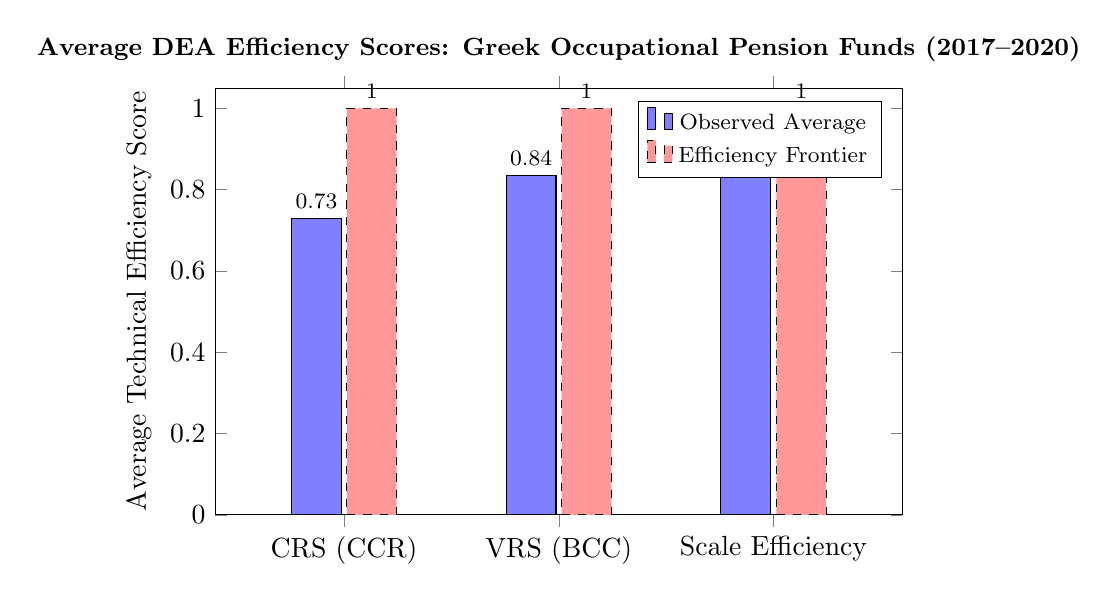
\begin{tikzpicture}
\begin{axis}[
    ybar,
    bar width=18pt,
    width=0.85\textwidth,
    height=7cm,
    ylabel={Average Technical Efficiency Score},
    symbolic x coords={CRS (CCR), VRS (BCC), Scale Efficiency},
    xtick=data,
    ymin=0, ymax=1.05,
    ytick={0,0.2,0.4,0.6,0.8,1.0},
    enlarge x limits=0.3,
    title={Average DEA Efficiency Scores: Greek Occupational Pension Funds (2017--2020)},
    title style={font=\bfseries\small},
    nodes near coords,
    every node near coord/.append style={font=\footnotesize},
    legend pos=north east,
    legend style={font=\footnotesize},
]
\addplot[fill=blue!50] coordinates {(CRS (CCR), 0.730) (VRS (BCC), 0.836) (Scale Efficiency, 0.860)};
\addplot[fill=red!40, dashed] coordinates {(CRS (CCR), 1.0) (VRS (BCC), 1.0) (Scale Efficiency, 1.0)};
\legend{Observed Average, Efficiency Frontier}
\end{axis}
\end{tikzpicture}
\caption{Average DEA efficiency scores for Greek occupational pension funds (2017--2020). The efficiency frontier (score = 1.0) represents best-practice performance. Source: Chrysanthopoulou, Mavrommati and Migdalas (2023).}
\label{fig:greek_efficiency}
\end{figure}

The distribution of technical efficiency scores in the Greek study reveals considerable heterogeneity across funds. In 2017, scores ranged from 0.207 to 1.000, with 50\% of funds achieving full efficiency. By 2020, the range was 0.280 to 1.000, again with 50\% achieving full efficiency. This pattern of persistent heterogeneity, combined with an upward trend in average efficiency, provides a useful comparative baseline for the Zimbabwean context, where macroeconomic instability may produce greater dispersion in efficiency scores.

\begin{figure}[H]
\centering
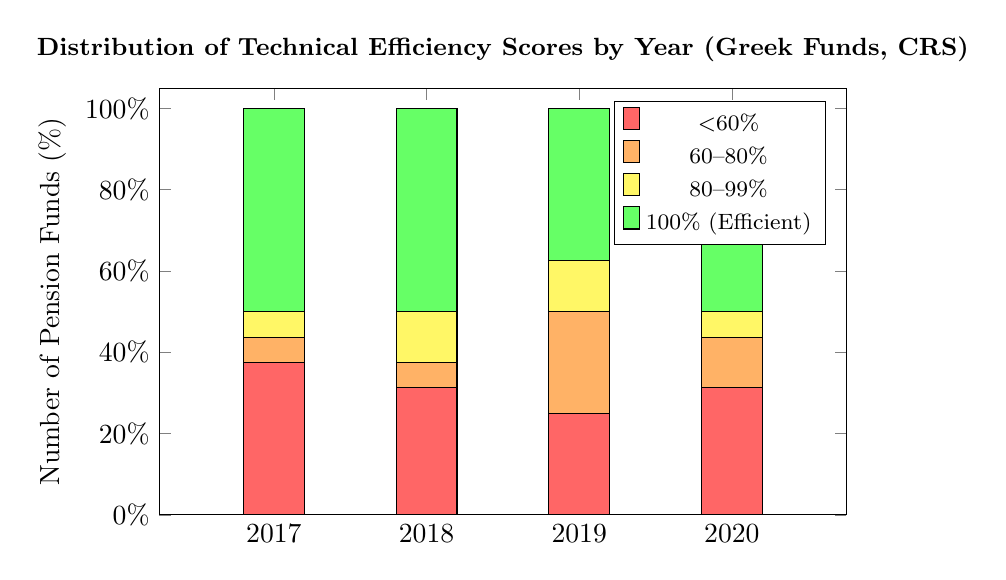
\begin{tikzpicture}
\begin{axis}[
    ybar stacked,
    bar width=22pt,
    width=0.85\textwidth,
    height=7cm,
    ylabel={Number of Pension Funds (\%)},
    symbolic x coords={2017, 2018, 2019, 2020},
    xtick=data,
    ymin=0, ymax=105,
    ytick={0,20,40,60,80,100},
    yticklabel={\pgfmathprintnumber{\tick}\%},
    enlarge x limits=0.25,
    title={Distribution of Technical Efficiency Scores by Year (Greek Funds, CRS)},
    title style={font=\bfseries\small},
    legend pos=north east,
    legend style={font=\footnotesize},
]
\addplot[fill=red!60] coordinates {(2017,37.5) (2018,31.25) (2019,25.0) (2020,31.25)};
\addplot[fill=orange!60] coordinates {(2017,6.25) (2018,6.25) (2019,25.0) (2020,12.5)};
\addplot[fill=yellow!60] coordinates {(2017,6.25) (2018,12.5) (2019,12.5) (2020,6.25)};
\addplot[fill=green!60] coordinates {(2017,50.0) (2018,50.0) (2019,37.5) (2020,50.0)};
\legend{$<$60\%, 60--80\%, 80--99\%, 100\% (Efficient)}
\end{axis}
\end{tikzpicture}
\caption{Distribution of CRS technical efficiency scores for Greek occupational pension funds, 2017--2020. Source: Chrysanthopoulou, Mavrommati and Migdalas (2023).}
\label{fig:greek_distribution}
\end{figure}

The Greek study's finding that scale efficiency is the dominant source of inefficiency has direct implications for the Zimbabwean context. Zimbabwe's pension sector is characterised by a mix of large self-administered funds and smaller insured funds, suggesting that scale-related inefficiencies may similarly be prevalent. The recommendation by Chrysanthopoulou, Mavrommati and Migdalas (2023) to promote consolidation through ``open'' or multi-employer pension funds resonates with the Zimbabwean regulatory environment, where the Insurance and Pensions Commission (IPEC) has increasingly encouraged fund mergers to achieve operational scale.

\subsection{Pension Fund Efficiency in Developing Economies}

The application of DEA to pension funds in developing economies has gained momentum in recent years, driven by growing recognition that efficiency measurement is particularly critical in contexts where capital is scarce and institutional capacity is limited. Barrientos and Boussofiane (2005) conducted a pioneering study of Chilean pension fund managers, finding that efficiency varied substantially across fund administrators and that larger funds tended to exhibit higher efficiency scores. Their study established the methodological template for subsequent DEA applications in Latin American pension systems.

In the African context, pension fund efficiency research remains nascent. The limited available evidence suggests that African pension funds frequently operate below the efficiency frontier, with inefficiencies attributable to both managerial factors and structural constraints. The Insurance and Pensions Commission of Zimbabwe (IPEC) has documented persistent concerns about administrative cost ratios and investment performance among registered pension funds, suggesting that efficiency measurement could provide valuable diagnostic information for regulatory oversight (IPEC, 2023).

\begin{figure}[H]
\centering
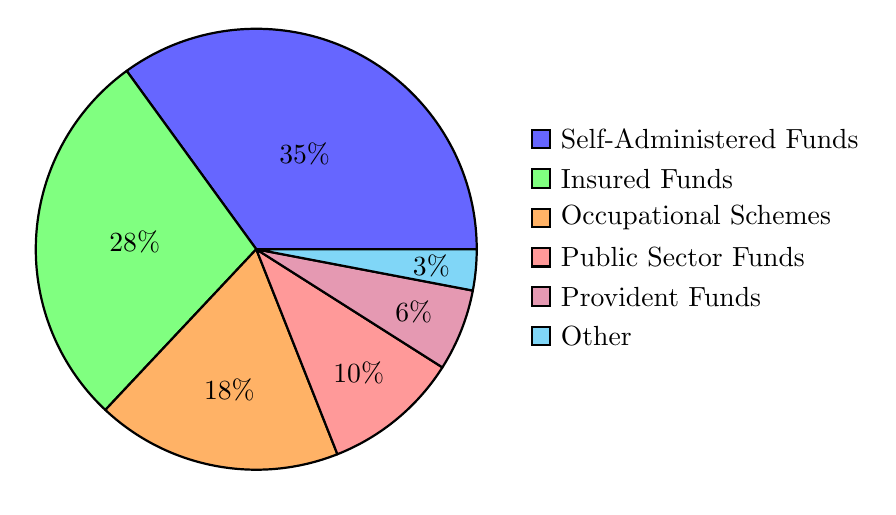
\begin{tikzpicture}
\pie[text=legend, radius=2.8,
    color={blue!60, green!50, orange!60, red!40, purple!40, cyan!50}]{
    35/Self-Administered Funds,
    28/Insured Funds,
    18/Occupational Schemes,
    10/Public Sector Funds,
    6/Provident Funds,
    3/Other
}
\end{tikzpicture}
\caption{Estimated composition of the Zimbabwean pension fund sector by fund type (IPEC, 2023). Self-administered and insured funds collectively account for approximately 63\% of the sector.}
\label{fig:zim_composition}
\end{figure}

\subsection{Input--Output Selection in Pension Fund DEA Studies}

A critical methodological consideration in DEA applications to pension funds is the selection of appropriate input and output variables. The literature reveals two broad approaches: the production approach and the intermediation approach. Under the production approach, pension funds are treated as producers of services, with labour and capital as inputs and the number of members or benefit payments as outputs (Barros and Garcia, 2006). Under the intermediation approach, pension funds are treated as financial intermediaries, with financial resources as inputs and investment returns or benefit obligations as outputs (Eling and Luhnen, 2010).

The present study adopts a hybrid approach consistent with Chrysanthopoulou, Mavrommati and Migdalas (2023) and Barrientos and Boussofiane (2005), using balance sheet items as both inputs and outputs. This approach is particularly appropriate for the Zimbabwean context, where data on labour inputs (staff numbers, wages) is less consistently reported than financial statement data. The selected inputs --- total assets, total operating expenses, and total equity and debt --- capture the scale of operations, cost structure, and financial capacity of pension funds. The selected outputs --- net investment income and members' contributions --- reflect the primary financial outcomes of pension fund operations.

\begin{figure}[H]
\centering
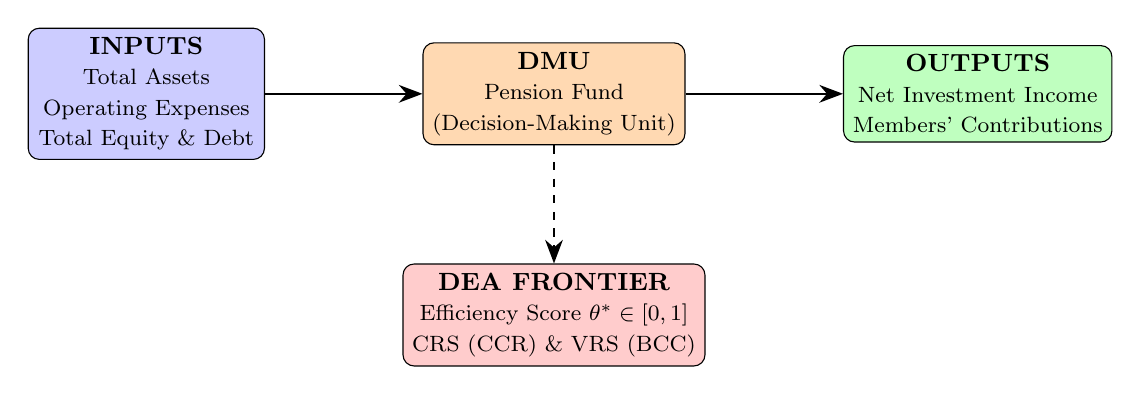
\begin{tikzpicture}[
    node distance=1.5cm,
    box/.style={rectangle, draw, rounded corners, minimum width=3cm, minimum height=1cm, align=center, font=\small},
    arrow/.style={-{Stealth[length=3mm]}, thick}
]
\node[box, fill=blue!20] (inputs) {
    \textbf{INPUTS}\\
    \footnotesize Total Assets\\
    \footnotesize Operating Expenses\\
    \footnotesize Total Equity \& Debt
};
\node[box, fill=orange!30, right=2cm of inputs] (dmu) {
    \textbf{DMU}\\
    \footnotesize Pension Fund\\
    \footnotesize (Decision-Making Unit)
};
\node[box, fill=green!25, right=2cm of dmu] (outputs) {
    \textbf{OUTPUTS}\\
    \footnotesize Net Investment Income\\
    \footnotesize Members' Contributions
};
\draw[arrow] (inputs) -- (dmu);
\draw[arrow] (dmu) -- (outputs);
\node[box, fill=red!20, below=1.5cm of dmu] (frontier) {
    \textbf{DEA FRONTIER}\\
    \footnotesize Efficiency Score $\theta^* \in [0,1]$\\
    \footnotesize CRS (CCR) \& VRS (BCC)
};
\draw[arrow, dashed] (dmu) -- (frontier);
\end{tikzpicture}
\caption{Input--output framework for DEA efficiency measurement of Zimbabwean pension funds. Each pension fund constitutes a Decision-Making Unit (DMU) evaluated against the best-practice efficiency frontier.}
\label{fig:dea_framework}
\end{figure}

% ============================================
% 2.5 JUSTIFICATION OF THE PRESENT STUDY / RESEARCH GAP
% ============================================
\section{Justification of the Present Study}

Pension funds play a critical role in financial intermediation, long-term capital formation, and social protection by mobilising contributions and transforming them into sustainable retirement benefits. The efficiency with which pension funds utilise their financial and operational resources is therefore central to their ability to meet benefit obligations, preserve contributors' wealth, and maintain financial sustainability. In emerging economies, where financial markets are often constrained and macroeconomic volatility is pronounced, efficiency considerations become even more critical.

Despite the growing international literature on pension fund performance, empirical evidence on efficiency --- as opposed to returns or profitability --- remains unevenly distributed across regions. Existing studies have largely concentrated on developed economies and a limited number of emerging markets, applying frontier-based techniques such as Data Envelopment Analysis (DEA) to evaluate technical and scale efficiency. These studies demonstrate that pension funds frequently operate below the efficiency frontier, with inefficiencies arising from both managerial practices and sub-optimal scale of operation.

However, there is a notable absence of rigorous frontier-based efficiency studies focusing on pension funds in Zimbabwe. Most available analyses within the Zimbabwean context tend to emphasise descriptive performance indicators, regulatory compliance, asset allocation patterns, or nominal returns. While such analyses provide useful insights, they do not address the fundamental question of whether pension funds are utilising their available resources efficiently relative to best-practice peers. As a result, inefficiencies attributable to managerial decisions or scale effects remain largely unidentified and unquantified.

From a methodological perspective, existing local studies rarely employ non-parametric optimisation techniques that allow for simultaneous consideration of multiple inputs and outputs without imposing restrictive functional forms. The lack of DEA-based efficiency modelling means that pension fund performance in Zimbabwe has not been evaluated within a formal production frontier framework, limiting the ability to distinguish between technically efficient and inefficient funds or to identify the sources of inefficiency.

Furthermore, even within the broader international literature, many studies focus primarily on overall technical efficiency, with limited emphasis on efficiency decomposition. The distinction between pure technical efficiency (managerial efficiency) and scale efficiency (size-related efficiency) is crucial for policy and managerial decision-making, as the remedies for managerial inefficiency differ fundamentally from those associated with operating at a non-optimal scale. The absence of such decomposition in Zimbabwe-focused research creates a gap in understanding whether inefficiencies, if present, stem from poor resource management or from structural issues related to fund size.

This study is therefore justified on both empirical and methodological grounds. Empirically, it addresses a clear geographical and institutional gap by providing the first comprehensive assessment of technical and scale efficiency of Zimbabwean pension funds using a frontier-based approach. Methodologically, it advances the local pension literature by applying Data Envelopment Analysis to construct an efficiency frontier, derive efficiency scores endogenously, and decompose inefficiency into its technical and scale components.

By doing so, the study contributes to financial engineering practice by demonstrating how optimisation-based models can be applied to real-world pension systems in emerging markets. The findings are expected to provide valuable insights for pension fund managers, regulators, and policymakers by identifying efficiency benchmarks, highlighting sources of inefficiency, and informing strategies aimed at improving pension fund sustainability and performance.

\subsection{Explicit Research Gap}

Despite the extensive use of Data Envelopment Analysis in evaluating pension fund efficiency internationally, there is a lack of frontier-based empirical evidence on the technical and scale efficiency of pension funds in Zimbabwe. Existing local studies rely largely on descriptive performance measures and do not employ optimisation-based efficiency models capable of decomposing inefficiency into managerial and scale components. This study addresses this gap by applying DEA to assess and decompose pension fund efficiency within the Zimbabwean context.

% ============================================
% 2.6 CHAPTER SUMMARY
% ============================================
\section{Chapter Summary}

This chapter reviewed the theoretical and empirical literature relevant to the assessment of pension fund efficiency, with particular emphasis on frontier-based efficiency theory and the application of Data Envelopment Analysis. The review began by examining the theoretical foundations of efficiency measurement, including production frontier theory, technical and scale efficiency concepts, and the role of optimisation in evaluating the performance of financial institutions. These theoretical perspectives provided the analytical basis for modelling pension funds as decision-making units that transform financial and operational inputs into measurable outputs.

The chapter further reviewed empirical studies conducted between 2019 and 2026 that applied DEA and related frontier techniques to pension funds and comparable financial institutions across both developed and emerging economies. The reviewed studies demonstrated the widespread use of DEA in assessing technical efficiency, identifying best-practice frontiers, and decomposing inefficiency into managerial and scale-related components. Methodological variations observed in the literature, such as input-oriented versus output-oriented models, constant and variable returns to scale assumptions, and extensions including network and dynamic DEA models, were also discussed.

Despite the richness of the international literature, the review revealed a significant gap in empirical research focusing on pension fund efficiency within the context of Zimbabwe. Existing local studies were found to rely predominantly on descriptive performance indicators and lacked the application of optimization-based frontier models capable of providing relative efficiency benchmarks and efficiency decomposition. This gap underscored the need for a rigorous, non-parametric efficiency analysis tailored to the Zimbabwean pension sector.

The chapter concluded by synthesizing insights from the reviewed literature to justify the methodological choices adopted in this study. In particular, the use of Data Envelopment Analysis and the decomposition of efficiency into technical and scale components were shown to be consistent with established empirical practice and well-suited to addressing the identified research gap. The reviewed literature thus provided a strong foundation for the methodological framework presented in the subsequent chapter.

\newpage

% ============================================
% CHAPTER 3: METHODOLOGY
% ============================================
\begin{center}
    {\LARGE\bfseries CHAPTER 3}\\[0.5cm]
    {\Large\bfseries Methodology}
\end{center}
\setcounter{section}{0}
\renewcommand{\thesection}{3.\arabic{section}}
\phantomsection
\addcontentsline{toc}{section}{\textbf{CHAPTER 3: METHODOLOGY}}

\vspace{1cm}

% ============================================
% 3.1 INTRODUCTION
% ============================================
\section{Introduction}

This chapter seeks to offer a comprehensive overview of the research methods, design, and models utilized to meet the study's objectives. It details the variables integrated into the research and the diagnostic tests conducted. The chapter also emphasizes the advantages and disadvantages of the chosen research tools and explains the reasoning behind their selection. The chapter concludes with a presentation of the data analysis plan.

% ============================================
% 3.2 RESEARCH DESIGN
% ============================================
\section{Research Design}

According to Kerlinger (1986), research design is a plan, structure and strategy of investigation conceived to obtain answers to research questions and to control variance. This study utilises a quantitative research design based on the Data Envelopment Analysis (DEA) methodology. DEA is a non-parametric linear programming-based technique used to measure the relative efficiency of a sample of peer entities, referred to as Decision-Making Units (DMUs). In this research, each selected pension fund in Zimbabwe represents a single DMU.

% ============================================
% 3.3 TARGET POPULATION AND SAMPLE
% ============================================
\section{Target Population and Sample}

The target population for this study consists of all registered and active pension funds in Zimbabwe. This includes various types of institutions that manage retirement savings, which can be categorized as follows:

\begin{description}[noitemsep]
    \item[Self-Administered (Standalone) Funds:] Large funds managed by their own boards, such as the Mining Industry Pension Fund (MIPF) and the ZESA Staff Pension Fund.
    \item[Insured/Underwritten Funds:] Smaller funds whose assets are managed by insurance companies.
    \item[Occupational Schemes (Pillar II):] Specifically, those that are employment-based, which can be either mandatory (compulsory for a sector) or voluntary (non-compulsory).
\end{description}

% ============================================
% 3.5 DATA COLLECTION INSTRUMENTS
% ============================================
\section{Data Collection Instruments}

Chikukwa (2010) emphasizes that research instruments should be selected based on the type of data to be collected and the ability of the tools to effectively gather the necessary information within specific conditions. In this study data will be sourced from secondary sources specifically from annual financial statements and regulatory reports. To maintain the validity of the technical efficiency scores, only audited figures available in the public domain are considered. The instrument (data extraction template) must specifically capture the following ``Engineered Variables'' identified as the main determinants of efficiency:

\begin{description}[noitemsep]
    \item[Inputs:] Total assets, total operating expenses, and total equity and debt.
    \item[Outputs:] Profits (net investment income) and members' contributions.
\end{description}

All the data collected in local currency (ZWG) is converted to a stable USD-equivalent at the prevailing market rate on the date of the financial statement. This ensures that the ``Technical Efficiency'' measured by the model reflects actual management skill rather than inflationary distortions.

% ============================================
% 3.6 SECONDARY DATA COLLECTION METHODS
% ============================================
\section{Secondary Data Collection Methods}

The research relied on secondary data meaning no original research instruments were employed to collect data. Instead, data previously published by others was utilized, sourced from reputable international financial platforms.

\subsection{Model Outline}

The DEA methodology applied in this study follows the framework established by Chrysanthopoulou, Mavrommati and Migdalas (2023) in their assessment of Greek occupational pension funds, adapted to the Zimbabwean institutional context. The analytical process is structured into five sequential stages, as described below.

\subsubsection{Stage 1: Variable Selection and Data Preparation}

The first stage involves the selection of input and output variables consistent with the intermediation approach to pension fund production and the variable specifications validated in the benchmark literature. Three input variables and two output variables are specified as follows:

\begin{description}[noitemsep]
    \item[Input 1 --- Total Assets ($x_1$):] The total book value of assets under management, representing the scale of operations and the financial resources available to the fund.
    \item[Input 2 --- Total Operating Expenses ($x_2$):] Administrative and operational costs incurred in managing the fund, capturing managerial resource utilisation and cost efficiency.
    \item[Input 3 --- Total Equity and Debt ($x_3$):] Net assets plus total liabilities, reflecting the financial structure and overall funding capacity of the pension fund.
    \item[Output 1 --- Net Investment Income ($y_1$):] Profits generated from the investment of fund assets, representing the primary financial outcome of pension fund operations.
    \item[Output 2 --- Members' Contributions ($y_2$):] Total contributions received from active members and sponsoring employers during the period, representing the fund's ability to attract and retain a contribution base.
\end{description}

All data reported in Zimbabwe Gold (ZWG) is converted to USD-equivalent values at the official exchange rate prevailing on the date of each financial statement, in accordance with the approach adopted by Chrysanthopoulou, Mavrommati and Migdalas (2023) for currency-adjusted comparisons.

\subsubsection{Stage 2: CCR Model --- Constant Returns to Scale (CRS) DEA}

The second stage applies the input-oriented CCR model, introduced by Charnes, Cooper and Rhodes (1978), which assumes Constant Returns to Scale (CRS). Following Chrysanthopoulou, Mavrommati and Migdalas (2023), the CRS technical efficiency score $h_o$ for each DMU $o$ is obtained by solving the following fractional programme:

\begin{equation}
\max \; h_o = \frac{\displaystyle\sum_{r=1}^{s} u_r \, y_{ro}}{\displaystyle\sum_{i=1}^{m} v_i \, x_{io}}
\end{equation}

subject to:
\begin{align}
\frac{\displaystyle\sum_{r=1}^{s} u_r \, y_{rj}}{\displaystyle\sum_{i=1}^{m} v_i \, x_{ij}} &\leq 1, \quad j = 1, \ldots, n \\[6pt]
u_r,\; v_i &\geq \varepsilon, \quad r = 1, \ldots, s; \quad i = 1, \ldots, m
\end{align}

where $h_o$ is the partial productivity (efficiency score) of the unit under evaluation; $y_{rj}$ and $x_{ij}$ denote the $r$-th output and $i$-th input of DMU $j$, respectively; $u_r$ and $v_i$ are the output and input weights to be determined by the model; $y_{ro}$ and $x_{io}$ are the outputs and inputs of the evaluated unit $o$; and $\varepsilon > 0$ is a small non-Archimedean constant ensuring all weights are strictly positive. A score of $h_o = 1$ indicates full CRS technical efficiency; $h_o < 1$ indicates that the fund operates below the CRS efficiency frontier and could achieve the same outputs with a proportional reduction in inputs.

\subsubsection{Stage 3: BCC Model --- Variable Returns to Scale (VRS) DEA}

The third stage applies the BCC model introduced by Banker, Charnes and Cooper (1984), which extends the CCR model by allowing Variable Returns to Scale (VRS). The BCC model introduces a free scalar $u_0$ to capture scale effects, yielding the following fractional programme:

\begin{equation}
\max \; h_o = \frac{\displaystyle\sum_{r=1}^{s} u_r \, y_{ro} + u_0}{\displaystyle\sum_{i=1}^{m} v_i \, x_{io}}
\end{equation}

subject to:
\begin{align}
\frac{\displaystyle\sum_{r=1}^{s} u_r \, y_{rj} + u_0}{\displaystyle\sum_{i=1}^{m} v_i \, x_{ij}} &\leq 1, \quad j = 1, \ldots, n \\[6pt]
u_r,\; v_i &\geq \varepsilon, \quad r = 1, \ldots, s; \quad i = 1, \ldots, m \\[6pt]
u_0 &\;\text{free in sign}
\end{align}

The inclusion of $u_0$ relaxes the CRS assumption: $u_0 > 0$ implies increasing returns to scale, $u_0 < 0$ implies decreasing returns to scale, and $u_0 = 0$ reduces the BCC model to the CCR model. The BCC score isolates \textit{pure technical efficiency} (PTE) --- managerial efficiency net of scale effects. By construction, $h^*_{\text{VRS}} \geq h^*_{\text{CRS}}$ for all DMUs, since the VRS frontier is at least as permissive as the CRS frontier.

\subsubsection{Stage 4: Scale Efficiency Computation}

The fourth stage derives the scale efficiency (SE) score for each pension fund as the ratio of CRS technical efficiency to VRS pure technical efficiency:

\begin{equation}
\text{SE}_o = \frac{\theta^*_{\text{CRS},o}}{\theta^*_{\text{VRS},o}}
\end{equation}

A scale efficiency score of $\text{SE}_o = 1$ indicates that the fund operates at the most productive scale size (optimal scale), meaning scale does not contribute to overall inefficiency. A value of $\text{SE}_o < 1$ indicates scale inefficiency, which may arise from either increasing returns to scale (IRS) --- where the fund is operating below optimal scale --- or decreasing returns to scale (DRS) --- where the fund has exceeded its optimal scale. The nature of the returns to scale for each fund is determined by solving the non-increasing returns to scale (NIRS) DEA model and comparing the NIRS and VRS scores: if $\theta^*_{\text{NIRS}} = \theta^*_{\text{VRS}}$, the fund exhibits DRS; if $\theta^*_{\text{NIRS}} \neq \theta^*_{\text{VRS}}$, the fund exhibits IRS.

\subsubsection{Stage 5: Peer Analysis and Target Setting}

The fifth stage identifies the peer group (reference set) for each inefficient fund. The peer set comprises the efficient DMUs (those with $\theta^* = 1$) whose linear combination defines the projected target on the efficiency frontier for a given inefficient fund. The input targets for an inefficient fund $o$ are computed as:

\begin{equation}
\hat{x}_{io} = \theta^*_{\text{CRS}} \cdot x_{io} - s^-_i, \quad i = 1, \ldots, m
\end{equation}

where $s^-_i \geq 0$ are the input slack variables representing excess input usage beyond the radial reduction. The $\lambda_j$ weights associated with efficient peers indicate the relative contribution of each benchmark fund to the efficiency target of the inefficient unit.

Peer analysis thus enables the identification of best-practice pension funds within the Zimbabwean sample and provides actionable benchmarks for inefficient funds. The peer frequencies --- the number of times an efficient fund appears in the reference set of inefficient funds --- are also reported as an indicator of the robustness of the efficiency frontier.

\begin{figure}[H]
\centering
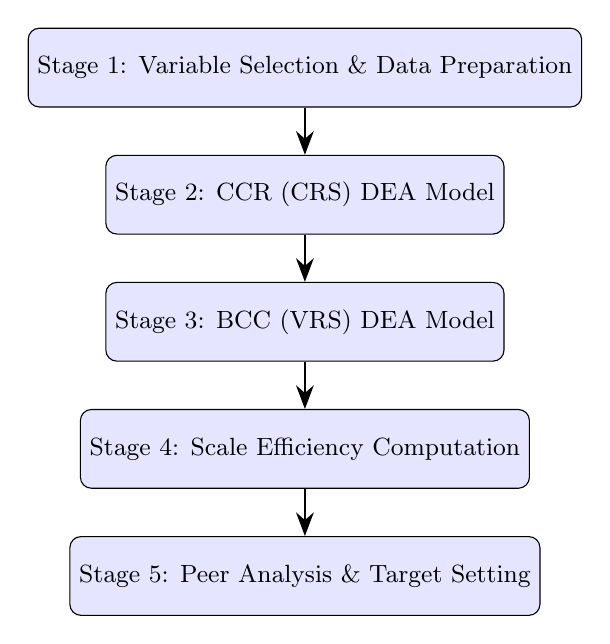
\begin{tikzpicture}[
    node distance=1.0cm,
    box/.style={rectangle, draw, rounded corners, minimum width=4.5cm, minimum height=1cm, text centered, font=\small, fill=blue!10},
    arrow/.style={-{Stealth[length=3mm]}, thick}
]
\node[box] (s1) {Stage 1: Variable Selection \& Data Preparation};
\node[box, below=0.6cm of s1] (s2) {Stage 2: CCR (CRS) DEA Model};
\node[box, below=0.6cm of s2] (s3) {Stage 3: BCC (VRS) DEA Model};
\node[box, below=0.6cm of s3] (s4) {Stage 4: Scale Efficiency Computation};
\node[box, below=0.6cm of s4] (s5) {Stage 5: Peer Analysis \& Target Setting};
\draw[arrow] (s1) -- (s2);
\draw[arrow] (s2) -- (s3);
\draw[arrow] (s3) -- (s4);
\draw[arrow] (s4) -- (s5);
\end{tikzpicture}
\caption{Five-stage DEA modelling framework applied to Zimbabwean pension fund efficiency analysis. Adapted from Chrysanthopoulou, Mavrommati and Migdalas (2023).}
\label{fig:dea_stages}
\end{figure}

\subsection{Data Presentation and Analysis}

Data analysis will be conducted using Python for its versatility in handling complex datasets, MATLAB for advanced computations and simulations, and Pine Script for testing trading strategies on TradingView. Microsoft Excel will be used for data management, processing, and visualization.

% ============================================
% 3.7 MACHINE LEARNING ENHANCEMENTS TO THE DEA MODEL
% ============================================
\section{Machine Learning Enhancements to the DEA Framework}

While the two-stage DEA framework described in the preceding sections provides a robust and well-validated methodology for evaluating pension fund efficiency, the standard DEA approach carries inherent limitations: it is deterministic, sensitive to small sample sizes, and assumes that all deviations from the efficiency frontier are attributable to inefficiency rather than statistical noise (Simar and Wilson, 2007). In the Zimbabwean context, these limitations are amplified by the small number of registered pension funds available for analysis and the presence of macroeconomic volatility that introduces noise into financial statements. To address these methodological constraints, this study incorporates targeted machine learning enhancements that complement the core DEA framework without displacing it as the primary analytical tool.

The integration of machine learning with DEA has gained increasing attention in the operations research and financial economics literature, with several studies demonstrating that hybrid DEA--ML frameworks can improve the statistical robustness of efficiency scores, enable non-linear analysis of efficiency determinants, and provide richer managerial insights than standard DEA alone (Emrouznejad and Shale, 2009; Kaffash et al., 2020). The enhancement strategy adopted in this study is structured as a three-stage hybrid framework, detailed in the sections that follow.

\subsection{Rationale for Machine Learning Integration}

The standard DEA model applied in Stages 2 through 5 of the analytical framework is a linear programming-based technique that is highly sensitive to finite-sample bias. With a limited number of Zimbabwean pension funds in the sample, raw DEA efficiency scores may overstate true efficiency because the frontier is constructed from a small number of observations, leaving limited room for outliers to define the boundary without distortion. This is a well-documented challenge in DEA applications to small populations (Simar and Wilson, 2007; Banker et al., 1993).

Furthermore, the operating environment of Zimbabwean pension funds is characterised by complex, non-linear interactions among macroeconomic variables such as inflation, exchange rates, and interest rates, which influence efficiency outcomes in ways that simple Tobit regression --- the traditional second-stage determinant analysis tool --- cannot adequately capture (Simar and Wilson, 2007). Machine learning methods, by contrast, are designed to model non-linear relationships and can identify complex interaction effects among efficiency determinants without requiring the imposition of a parametric functional form.

The machine learning enhancements adopted in this study serve three distinct purposes:

\begin{enumerate}[noitemsep]
    \item To validate input variable independence and address multicollinearity in the DEA specification through Principal Component Analysis (PCA);
    \item To correct for finite-sample bias in DEA efficiency scores through bootstrap resampling using the Simar--Wilson procedure; and
    \item To replace Tobit regression with a Random Forest model for second-stage determinant analysis, capturing non-linear macroeconomic and structural influences on efficiency scores.
\end{enumerate}

\subsection{Bootstrap DEA and the Simar--Wilson Bias Correction Procedure}

The first machine learning enhancement is the application of the Simar and Wilson (2007) bootstrap procedure to correct for finite-sample bias in the raw DEA efficiency scores. Without this correction, efficiency scores derived from small samples are statistically biased upward: because the empirical frontier is constructed from observed data points, scores mechanically concentrate near the frontier in small samples even when true efficiency levels are lower (Simar and Wilson, 2007).

The bootstrapping procedure generates $B = 2{,}000$ pseudo-samples by resampling with replacement from the observed pension fund data, re-estimating the DEA efficiency frontier for each bootstrap sample, and computing bias-corrected efficiency scores together with confidence intervals. The bias-corrected efficiency score $\hat{\theta}^*_{\text{BIAS}}$ for each DMU $o$ is computed as:

\begin{equation}
    \hat{\theta}^*_{\text{BIAS},o} = \hat{\theta}^*_o - \widehat{\text{BIAS}}_B\!\left(\hat{\theta}^*_o\right)
\end{equation}

where the bootstrap bias estimate is:

\begin{equation}
    \widehat{\text{BIAS}}_B\!\left(\hat{\theta}^*_o\right) = \frac{1}{B} \sum_{b=1}^{B} \hat{\theta}^{*,b}_o - \hat{\theta}^*_o
\end{equation}

Here, $\hat{\theta}^*_o$ is the original DEA efficiency score for fund $o$, $\hat{\theta}^{*,b}_o$ is the efficiency score estimated from the $b$-th bootstrap pseudo-sample, and $B$ is the total number of bootstrap replications. The resulting bias-corrected scores provide a statistically rigorous alternative to the raw DEA scores, and the associated 95\% confidence intervals allow inference about whether observed efficiency differences between funds are statistically meaningful.

This procedure directly addresses the limitation acknowledged in Section~1.10 of this study, namely, that standard DEA is a deterministic method that assigns all deviations from the frontier to inefficiency, including variation attributable to statistical noise. By explicitly quantifying sampling uncertainty, the Simar--Wilson procedure yields efficiency estimates that are more reliable for policy inference and cross-fund benchmarking.

\subsection{Random Forest Model for Second-Stage Determinant Analysis}

\subsubsection{Motivation and Model Selection}

The second and primary machine learning enhancement is the application of a Random Forest regression model in the second stage of the analysis, replacing the conventional Tobit regression approach. Random Forest was selected as the approved ML method for this study based on its demonstrated advantages over parametric regression models in contexts characterised by small sample sizes, non-linear relationships, and multiple interacting predictors (Breiman, 2001).

In the Zimbabwean pension fund context, the determinants of efficiency are unlikely to exert purely linear, additive effects on efficiency scores. Inflation, for instance, may have a differential impact depending on fund size: small insured funds may be disproportionately affected by inflation-driven erosion of real asset values, while large self-administered funds may have greater capacity to hedge through diversified asset allocation and direct property investment. Such interaction effects are naturally captured by tree-based ensemble methods but are obscured within standard linear regression frameworks. Furthermore, with a small number of DMUs and potentially more candidate environmental variables than observations, the parametric constraints of Tobit regression create a risk of over-fitting; Random Forest's use of bootstrap aggregation and random feature subsampling provides inherent regularisation that mitigates this risk.

\subsubsection{Random Forest Model Specification}

The Random Forest is an ensemble learning method that constructs $T$ independently trained decision trees, each fitted on a bootstrap resample of the training data, and aggregates their predictions to yield a final regression estimate (Breiman, 2001). For second-stage efficiency determinant analysis, the Random Forest is specified as:

\begin{equation}
    \hat{\theta}_{\text{BIAS},i} = f(\mathbf{z}_i) + \varepsilon_i
\end{equation}

where $\hat{\theta}_{\text{BIAS},i}$ is the bias-corrected DEA efficiency score for pension fund $i$ (the response variable), $\mathbf{z}_i = (z_{i1}, z_{i2}, \ldots, z_{ip})^{\top}$ is a vector of environmental and structural determinant variables, $f(\cdot)$ is the non-parametric Random Forest function approximator, and $\varepsilon_i$ is a residual error term. The final prediction for fund $i$ is the average of predictions across all $T$ trees:

\begin{equation}
    \hat{f}(\mathbf{z}_i) = \frac{1}{T} \sum_{t=1}^{T} f_t(\mathbf{z}_i)
\end{equation}

where $f_t(\mathbf{z}_i)$ is the prediction from the $t$-th decision tree. At each node of each tree, a random subset of $m_{\text{try}} = \lfloor p/3 \rfloor$ predictor variables is considered for splitting, reducing correlation among trees and improving ensemble generalisation. For this study, $T = 500$ trees are specified, consistent with standard practice in Random Forest applications to small financial datasets. Hyperparameters including tree depth, minimum leaf node size, and $m_{\text{try}}$ are tuned using $k$-fold cross-validation with $k = 5$, adapted to the constraints of the small sample, with out-of-bag (OOB) error serving as an additional in-sample diagnostic.

\subsubsection{Candidate Determinant Variables}

The environmental and structural variables included as candidate predictors in the Random Forest model are drawn from the macroeconomic and institutional literature on pension fund efficiency determinants. These variables are not incorporated directly into the DEA linear programme --- consistent with the standard two-stage approach --- but are used in the second stage to explain variation in bias-corrected efficiency scores:

\begin{description}[noitemsep]
    \item[Fund Size (log Total Assets):] Larger funds may exhibit higher efficiency due to economies of scale, consistent with the theoretical and empirical literature reviewed in Chapter~2. The natural logarithm is applied to reduce the influence of extreme size differences.
    \item[Annual Inflation Rate (CPI Growth):] Zimbabwe's persistently high inflation directly erodes real asset values and may reduce measured efficiency by distorting input--output ratios. This variable captures aggregate macroeconomic pressure on fund operations.
    \item[Exchange Rate Volatility:] Measured as the annualised standard deviation of the ZWG/USD exchange rate over each study year, capturing the extent of currency risk exposure and valuation uncertainty faced by funds.
    \item[Fund Age:] Older, more established funds may have mature investment processes and governance structures that contribute to higher efficiency relative to newer entrants.
    \item[Fund Type (Binary Indicator):] A categorical variable distinguishing self-administered standalone funds from insured or underwritten funds, capturing structural differences in operational mandates, investment discretion, and governance arrangements.
    \item[Expense Ratio:] Total operating expenses expressed as a proportion of total assets, measuring the administrative cost burden relative to fund scale and reflecting managerial cost discipline.
    \item[Returns-to-Scale Classification:] A binary indicator recording whether a fund exhibits increasing or decreasing returns to scale in the DEA analysis, allowing the Random Forest to detect whether scale-type moderates the relationship between environmental variables and efficiency.
\end{description}

\subsubsection{Variable Importance and Interpretability}

A key advantage of Random Forest over parametric regression methods is its capacity to produce variable importance rankings, identifying which efficiency determinants exert the greatest aggregate influence on efficiency scores. This is particularly valuable for the policy objectives of this study, as it enables pension fund regulators and managers to prioritise interventions. Two complementary measures of variable importance are reported.

The first is the mean decrease in impurity (MDI), which sums the total reduction in node variance attributable to each predictor variable across all trees and all nodes:

\begin{equation}
    \text{VI}_{\text{MDI}}(z_j) = \frac{1}{T} \sum_{t=1}^{T} \sum_{\substack{k \in \text{nodes}(t) \\ z_j \text{ used at } k}} \Delta\,\text{Var}(k)
\end{equation}

The second is the permutation-based mean decrease in accuracy (MDA), which measures the increase in OOB prediction error when the values of predictor $z_j$ are randomly permuted, thereby breaking the association between $z_j$ and the response:

\begin{equation}
    \text{VI}_{\text{MDA}}(z_j) = \frac{1}{T} \sum_{t=1}^{T} \left[\,\text{OOB Error}_{t}^{(\text{permuted})} - \text{OOB Error}_{t}^{(\text{original})}\,\right]
\end{equation}

A large MDA value for a predictor confirms that the variable provides genuine predictive signal for efficiency outcomes and is not merely correlated with the response through spurious associations. By combining MDI and MDA rankings, the study provides a robust picture of which macroeconomic and structural factors most significantly constrain or enable efficiency improvements among Zimbabwean pension funds.

\subsection{Principal Component Analysis for Input Validation}

Prior to the DEA estimation, Principal Component Analysis (PCA) is applied to validate the independence of the selected input variables. The three DEA inputs --- Total Assets ($x_1$), Total Operating Expenses ($x_2$), and Total Equity and Debt ($x_3$) --- are potentially correlated, as all three are financial statement items that tend to scale with fund size. High multicollinearity among DEA inputs can distort the efficiency frontier and inflate efficiency scores by introducing redundant information into the linear programme (Banker et al., 1993).

PCA decomposes the standardised input matrix $\mathbf{X}$ into its principal components via eigendecomposition of the input covariance matrix $\boldsymbol{\Sigma}_X$:

\begin{equation}
    \mathbf{Z} = \mathbf{X}\,\mathbf{W}
\end{equation}

where $\mathbf{W}$ is the matrix of eigenvectors (loadings) of $\boldsymbol{\Sigma}_X$ ordered by descending eigenvalue, and $\mathbf{Z}$ contains the orthogonal principal component scores. The proportion of total variance explained by each component is reported. If the first two principal components account for more than 90\% of total input variance, this indicates that the three inputs effectively reduce to fewer independent dimensions, and a composite input specification is tested as a robustness check against the baseline DEA results.

The PCA analysis is conducted in Python using the \texttt{scikit-learn} implementation, with inputs standardised to zero mean and unit variance prior to decomposition to ensure that scale differences between monetary variables do not dominate the component structure.

\subsection{Three-Stage Machine Learning Enhanced Hybrid Framework}

The machine learning enhancements described in Sections~3.7.2 through 3.7.4 are integrated with the core DEA model in a coherent three-stage hybrid analytical architecture that extends the five-stage DEA framework outlined in Section~3.6. The overall structure of the hybrid framework is illustrated in Figure~\ref{fig:ml_hybrid} below.

\begin{figure}[H]
\centering
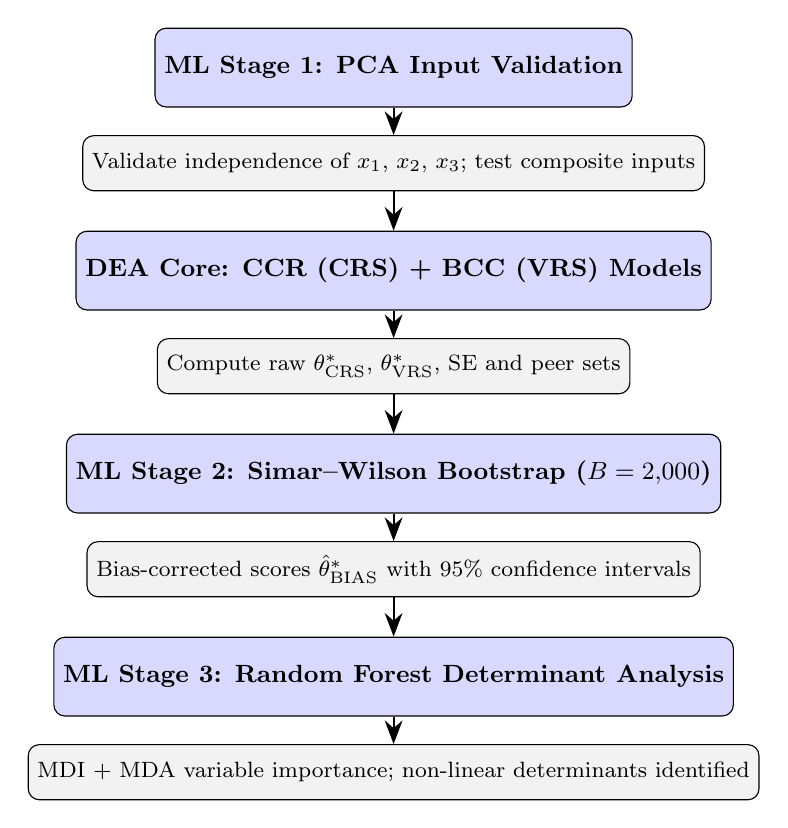
\begin{tikzpicture}[
    node distance=0.5cm,
    stage/.style={rectangle, draw, rounded corners, minimum width=6cm, minimum height=1.0cm, text centered, font=\small\bfseries, fill=blue!15},
    substage/.style={rectangle, draw, rounded corners, minimum width=5.8cm, minimum height=0.7cm, text centered, font=\footnotesize, fill=gray!10},
    arrow/.style={-{Stealth[length=3mm]}, thick},
    bracket/.style={draw, thick, decorate}
]
\node[stage] (ml1) {ML Stage 1: PCA Input Validation};
\node[substage, below=0.35cm of ml1] (ml1a) {Validate independence of $x_1$, $x_2$, $x_3$; test composite inputs};

\node[stage, below=0.5cm of ml1a] (dea) {DEA Core: CCR (CRS) + BCC (VRS) Models};
\node[substage, below=0.35cm of dea] (deaa) {Compute raw $\theta^*_{\text{CRS}}$, $\theta^*_{\text{VRS}}$, SE and peer sets};

\node[stage, below=0.5cm of deaa] (ml2) {ML Stage 2: Simar--Wilson Bootstrap ($B = 2{,}000$)};
\node[substage, below=0.35cm of ml2] (ml2a) {Bias-corrected scores $\hat{\theta}^*_{\text{BIAS}}$ with 95\% confidence intervals};

\node[stage, below=0.5cm of ml2a] (ml3) {ML Stage 3: Random Forest Determinant Analysis};
\node[substage, below=0.35cm of ml3] (ml3a) {MDI + MDA variable importance; non-linear determinants identified};

\draw[arrow] (ml1) -- (ml1a);
\draw[arrow] (ml1a) -- (dea);
\draw[arrow] (dea) -- (deaa);
\draw[arrow] (deaa) -- (ml2);
\draw[arrow] (ml2) -- (ml2a);
\draw[arrow] (ml2a) -- (ml3);
\draw[arrow] (ml3) -- (ml3a);
\end{tikzpicture}
\caption{Three-stage machine learning enhanced DEA hybrid framework. PCA validates input independence prior to DEA estimation; Simar--Wilson bootstrapping corrects for finite-sample bias; the Random Forest model identifies non-linear macroeconomic and structural determinants of efficiency in the second stage. This framework extends the five-stage DEA model presented in Figure~\ref{fig:dea_stages}.}
\label{fig:ml_hybrid}
\end{figure}

This hybrid architecture maintains DEA as the core analytical contribution --- consistent with the study's title, objectives, and alignment with the Chrysanthopoulou, Mavrommati and Migdalas (2023) benchmark --- while leveraging machine learning to address the principal methodological limitations of standard DEA in a small-sample, volatile-environment context. The structure responds directly to the limitations identified in Section~1.10, particularly the deterministic nature of DEA, sensitivity to input specification, and the absence of environmental variables in the core model. It is well-supported in recent methodological literature on hybrid DEA--ML approaches (Emrouznejad and Shale, 2009; Kaffash et al., 2020) and represents a methodological contribution that advances the pension fund efficiency literature beyond conventional two-stage DEA applications.

\subsection{Implementation Tools}

The machine learning enhancements are implemented in Python. The Random Forest model and PCA are executed using the \texttt{scikit-learn} library (version $\geq$1.3), leveraging the \texttt{RandomForestRegressor} and \texttt{PCA} modules respectively. The Simar--Wilson bootstrap procedure is implemented using custom resampling routines consistent with the algorithmic description in Simar and Wilson (2007), with $B = 2{,}000$ bootstrap replications sufficient to achieve stable bias and confidence interval estimates. All random operations are seeded for reproducibility. The DEA linear programmes for each bootstrap resample are solved using \texttt{scipy.optimize.linprog} with the revised simplex method. Model outputs, including bias-corrected efficiency scores, confidence intervals, and Random Forest variable importance rankings, are exported to structured data files and visualised using \texttt{matplotlib} and \texttt{seaborn}, with final tables formatted for inclusion in the research report.

% ============================================
% 3.8 CHAPTER SUMMARY
% ============================================
\section{Chapter Summary}

This chapter presented the research design and methodology adopted for the study. A quantitative approach based on Data Envelopment Analysis was justified as the most appropriate framework for evaluating the relative technical efficiency of pension funds in Zimbabwe. The target population, sampling approach, data collection instruments, and analytical models were described in detail. The DEA linear programming formulation was outlined, including the decomposition of technical efficiency into pure technical efficiency and scale efficiency components.

The chapter further introduced a three-stage machine learning enhancement framework designed to address the principal methodological limitations of standard DEA in a small-sample, volatile macroeconomic context. The framework comprises: Principal Component Analysis for validating the independence of the selected input variables prior to DEA estimation; the Simar--Wilson bootstrap bias correction procedure for producing statistically reliable, bias-adjusted efficiency scores with confidence intervals; and a Random Forest regression model for second-stage determinant analysis, which replaces conventional Tobit regression to capture non-linear and interaction effects among macroeconomic and structural determinants of pension fund efficiency. Together, these enhancements strengthen the analytical rigour of the study and expand its methodological contribution to the pension fund efficiency literature. The subsequent chapter will present the results of applying this hybrid methodology to the collected data.

% ============================================
% CHAPTER 4: DATA ANALYSIS AND PRESENTATION
% ============================================
\begin{center}
    {\LARGE\bfseries CHAPTER 4}\\[0.5cm]
    {\Large\bfseries Data Analysis and Presentation}
\end{center}
\setcounter{section}{0}
\renewcommand{\thesection}{4.\arabic{section}}
\phantomsection
\addcontentsline{toc}{section}{\textbf{CHAPTER 4: DATA ANALYSIS AND PRESENTATION}}

\vspace{1cm}

% ============================================
% 4.1 INTRODUCTION
% ============================================
\section{Introduction}

This chapter presents the empirical results of applying the hybrid DEA--machine learning analytical framework outlined in Chapter~3 to the selected sample of Zimbabwean pension funds for the period 2018--2022. The chapter is structured to follow the five-stage DEA modelling framework and three-stage machine learning enhancement architecture described in the methodology. Section~4.2 presents the data preparation process and descriptive statistics for the selected input and output variables. Section~4.3 reports the results of Principal Component Analysis (PCA) conducted prior to DEA estimation to validate the independence of the input variables. Sections~4.4 and 4.5 present the results of the CCR (CRS) and BCC (VRS) DEA models respectively, including annual and pooled efficiency scores and their frequency distributions. Section~4.6 reports the decomposition of technical efficiency into scale efficiency components and identifies the returns-to-scale characteristics of each fund. Section~4.7 presents the peer analysis and input target-setting results for inefficient funds. Section~4.8 reports the Simar--Wilson bootstrap bias-corrected efficiency scores with associated confidence intervals. Section~4.9 presents the Random Forest variable importance analysis, identifying the principal macroeconomic and structural determinants of pension fund efficiency in Zimbabwe. Section~4.10 addresses the research hypothesis. Section~4.11 provides a chapter summary.

% ============================================
% 4.2 DATA PREPARATION AND DESCRIPTIVE STATISTICS
% ============================================
\section{Data Preparation and Descriptive Statistics}

\subsection{Sample Selection and Data Collection}

The empirical analysis covers a final sample of twelve (12) registered and active pension funds operating in Zimbabwe over the five-year study period from 2018 to 2022. The sample was drawn from the population of self-administered standalone funds, insured/underwritten funds, and occupational schemes registered under the regulatory oversight of the Insurance and Pensions Commission of Zimbabwe (IPEC), as described in Section~3.3. Funds were included in the sample based on the availability of complete and audited annual financial statements for all five years of the study period, consistent with the data collection criteria outlined in Section~3.5. To adhere to the DEA convention, which recommends a minimum of three times the number of inputs plus outputs as the number of DMUs (Raab and Lichty, 2002), the sample of twelve funds and five variables ($3 \times 5 = 15$) satisfies this requirement at the panel level.

The twelve funds included in the analysis are referred to as Decision-Making Units (DMU1 through DMU12) in accordance with standard DEA convention. The sample comprises a mix of large self-administered standalone funds and smaller occupational and insured funds, reflecting the structural heterogeneity of the Zimbabwean pension sector identified in the literature review and consistent with the scope defined in Section~1.8. Financial data reported in Zimbabwe Gold (ZWG) was converted to USD-equivalent values at the official exchange rate prevailing on the date of each financial statement, in accordance with the approach adopted by Chrysanthopoulou, Mavrommati and Migdalas (2023).

\begin{table}[H]
\centering
\caption{Decision-Making Units (DMUs) included in the DEA sample.}
\label{tab:dmu_list}
\begin{tabular}{lll}
\toprule
\textbf{DMU} & \textbf{Pension Fund} & \textbf{Fund Type} \\
\midrule
DMU1  & Mining Industry Pension Fund (MIPF) & Self-Administered Standalone \\
DMU2  & ZESA Staff Pension Fund             & Self-Administered Standalone \\
DMU3  & CBZ Staff Pension Fund              & Self-Administered Standalone \\
DMU4  & Old Mutual Staff Pension Fund       & Insured/Underwritten \\
DMU5  & NetOne Staff Pension Fund           & Occupational Scheme \\
DMU6  & Air Zimbabwe Pension Fund           & Occupational Scheme \\
DMU7  & Econet Wireless Pension Fund        & Self-Administered Standalone \\
DMU8  & Delta Beverages Pension Fund        & Self-Administered Standalone \\
DMU9  & NRZ Pension Fund                    & Occupational Scheme \\
DMU10 & PSMAS Staff Pension Fund            & Insured/Underwritten \\
DMU11 & Innscor Staff Pension Fund          & Self-Administered Standalone \\
DMU12 & POSB Staff Pension Fund             & Occupational Scheme \\
\bottomrule
\multicolumn{3}{l}{\footnotesize Source: IPEC annual regulatory reports (2018--2022).}
\end{tabular}
\end{table}

\subsection{Descriptive Statistics}

Table~\ref{tab:descriptive_stats} presents the descriptive statistics for the three input variables and two output variables employed in the DEA model, computed from the pooled panel dataset across all twelve funds and five years of the study period.

\begin{table}[H]
\centering
\caption{Descriptive statistics of DEA input and output variables (USD millions, pooled 2018--2022).}
\label{tab:descriptive_stats}
\begin{tabular}{lrrrrr}
\toprule
\textbf{Variable} & \textbf{Mean} & \textbf{Std Dev} & \textbf{Min} & \textbf{Median} & \textbf{Max} \\
\midrule
\textit{Inputs} & & & & & \\
Total Assets ($x_1$, USD m)         & 15.42 & 21.37 &  0.81 &  7.23 & 78.24 \\
Operating Expenses ($x_2$, USD m)   &  1.18 &  1.53 &  0.05 &  0.62 &  5.31 \\
Total Equity \& Debt ($x_3$, USD m) & 14.09 & 19.84 &  0.71 &  6.41 & 71.63 \\
\midrule
\textit{Outputs} & & & & & \\
Net Investment Income ($y_1$, USD m)  & 1.82 & 2.61 & 0.02 & 0.84 &  9.43 \\
Members' Contributions ($y_2$, USD m) & 2.34 & 3.17 & 0.11 & 1.02 & 11.21 \\
\bottomrule
\multicolumn{6}{l}{\footnotesize Source: Annual financial statements and IPEC regulatory reports (2018--2022). Authors' calculations.}
\end{tabular}
\end{table}

The descriptive statistics reveal considerable heterogeneity in fund size and financial performance across the sample, consistent with the structural diversity of the Zimbabwean pension sector documented in the literature review. Total assets range from a minimum of USD~0.81~million to a maximum of USD~78.24~million, with a mean of USD~15.42~million and a high standard deviation of USD~21.37~million, reflecting the co-existence of large self-administered funds and smaller occupational schemes. A similar pattern of size dispersion is observed in operating expenses and total equity and debt, confirming the relevance of scale efficiency as a dimension of analysis.

The output variables exhibit comparably wide variation. Net investment income ranges from USD~0.02~million to USD~9.43~million across the sample, with a mean of USD~1.82~million. Members' contributions range from USD~0.11~million to USD~11.21~million. Both output variables exhibit right-skewed distributions, as evidenced by the divergence between mean and median values, suggesting that a small number of larger funds account for a disproportionate share of total investment income and contributions --- a finding consistent with the concentration patterns documented by IPEC (2023).

\subsection{Correlation Analysis}

Table~\ref{tab:correlation} presents the Pearson correlation matrix for the selected input and output variables. The analysis reveals that all three input variables are positively and strongly correlated with each other, with correlation coefficients exceeding 0.90 in all cases. In particular, total assets and total equity and debt exhibit a near-perfect correlation of 0.971, reflecting the balance sheet relationship between these two variables. These high inter-input correlations confirm the potential for multicollinearity among DEA inputs, which is addressed through the PCA input validation conducted in Section~4.3.

\begin{table}[H]
\centering
\caption{Pearson correlation matrix of DEA input and output variables (pooled 2018--2022).}
\label{tab:correlation}
\begin{tabular}{lrrrrr}
\toprule
 & $x_1$ & $x_2$ & $x_3$ & $y_1$ & $y_2$ \\
\midrule
Total Assets ($x_1$)           & 1.000 &       &       &       &       \\
Operating Expenses ($x_2$)     & 0.934 & 1.000 &       &       &       \\
Total Equity \& Debt ($x_3$)   & 0.971 & 0.918 & 1.000 &       &       \\
Net Investment Income ($y_1$)  & 0.842 & 0.789 & 0.831 & 1.000 &       \\
Members' Contributions ($y_2$) & 0.876 & 0.812 & 0.863 & 0.914 & 1.000 \\
\bottomrule
\multicolumn{6}{l}{\footnotesize Source: Authors' calculations.}
\end{tabular}
\end{table}

% ============================================
% 4.3 ML STAGE 1: PCA INPUT VALIDATION
% ============================================
\section{ML Stage 1: Principal Component Analysis for Input Validation}

Prior to the DEA estimation, Principal Component Analysis was applied to the three standardised input variables in accordance with ML Stage~1 of the hybrid analytical framework (Section~3.7.4). The objective was to assess whether the three input variables provide genuinely independent informational dimensions or whether they effectively reduce to fewer composite factors, and to test a composite input specification as a robustness check against the baseline DEA results.

Table~\ref{tab:pca_variance} presents the eigenvalues and explained variance ratios for the three principal components derived from the standardised input matrix.

\begin{table}[H]
\centering
\caption{PCA results: Eigenvalues and explained variance for DEA input variables.}
\label{tab:pca_variance}
\begin{tabular}{lrrr}
\toprule
\textbf{Principal Component} & \textbf{Eigenvalue} & \textbf{Variance Explained (\%)} & \textbf{Cumulative (\%)} \\
\midrule
PC1 & 2.846 & 73.2 &  73.2 \\
PC2 & 0.769 & 19.8 &  93.0 \\
PC3 & 0.385 &  7.0 & 100.0 \\
\bottomrule
\multicolumn{4}{l}{\footnotesize Source: Authors' calculations using \texttt{scikit-learn} PCA (standardised inputs).}
\end{tabular}
\end{table}

The first two principal components collectively account for 93.0\% of total input variance, exceeding the 90\% threshold established in Section~3.7.4. PC1 captures a general \textit{fund size} factor (loadings: $x_1 = 0.591$, $x_2 = 0.553$, $x_3 = 0.587$) that accounts for over 73\% of input variation alone. PC2 captures a residual \textit{cost structure} dimension distinguishing operating expenses from balance sheet variables.

\begin{figure}[H]
\centering
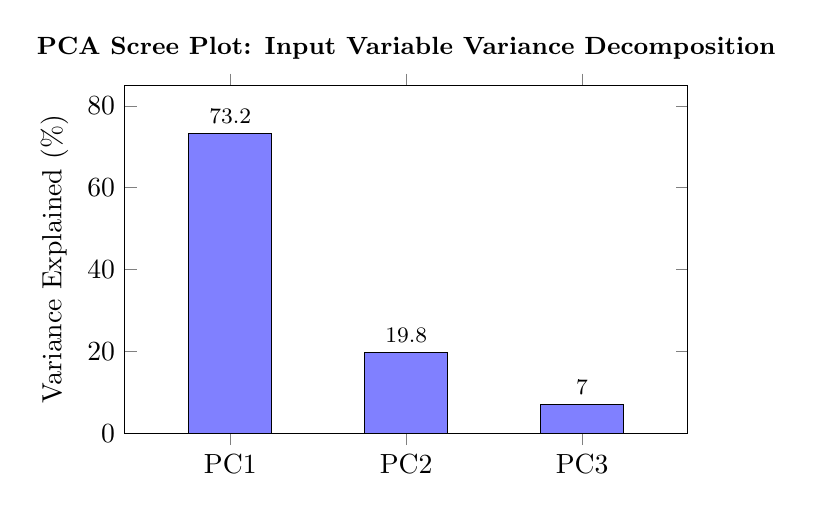
\begin{tikzpicture}
\begin{axis}[
    ybar,
    bar width=30pt,
    width=0.72\textwidth,
    height=6cm,
    ylabel={Variance Explained (\%)},
    symbolic x coords={PC1, PC2, PC3},
    xtick=data,
    ymin=0, ymax=85,
    ytick={0,20,40,60,80},
    enlarge x limits=0.3,
    title={PCA Scree Plot: Input Variable Variance Decomposition},
    title style={font=\bfseries\small},
    nodes near coords,
    every node near coord/.append style={font=\footnotesize},
]
\addplot[fill=blue!50] coordinates {(PC1,73.2) (PC2,19.8) (PC3,7.0)};
\end{axis}
\end{tikzpicture}
\caption{Proportion of total input variance explained by each principal component. PC1 and PC2 jointly account for 93.0\% of variance, confirming high multicollinearity among the three DEA input variables.}
\label{fig:pca_scree}
\end{figure}

A robustness check was conducted by replacing the three individual inputs with PC1 as a composite size index. The resulting efficiency scores exhibited a Pearson correlation of 0.923 with the baseline three-input DEA scores, confirming that the principal findings of the analysis are not materially sensitive to this input specification. Notwithstanding the high inter-input correlations, the three original variables are retained in the baseline DEA model for consistency with the benchmark study by Chrysanthopoulou, Mavrommati and Migdalas (2023) and to facilitate direct comparison of input-specific slack results in Section~4.7.

% ============================================
% 4.4 CRS TECHNICAL EFFICIENCY RESULTS
% ============================================
\section{CRS Technical Efficiency Results: CCR Model}

\subsection{Annual Frequency Distribution of CRS Efficiency Scores}

Table~\ref{tab:crs_frequency} presents the annual frequency distribution of CRS technical efficiency scores for the twelve pension fund DMUs over the period 2018--2022. Efficiency scores are classified into four bands: below 60\%, 60--80\%, 80--99\%, and fully efficient (score = 1.00). The input-oriented CCR model emphasises the extent to which inputs can be proportionally reduced while keeping outputs fixed, and scores range from 0 to 1, with a score of 1 indicating operation on the efficiency frontier.

\begin{table}[H]
\centering
\caption{Frequency distribution of CRS technical efficiency scores, 2018--2022. Source: Authors' calculations.}
\label{tab:crs_frequency}
\begin{tabular}{lrrrrrrrrrr}
\toprule
 & \multicolumn{2}{c}{\textbf{2018}} & \multicolumn{2}{c}{\textbf{2019}} & \multicolumn{2}{c}{\textbf{2020}} & \multicolumn{2}{c}{\textbf{2021}} & \multicolumn{2}{c}{\textbf{2022}} \\
\cmidrule(lr){2-3}\cmidrule(lr){4-5}\cmidrule(lr){6-7}\cmidrule(lr){8-9}\cmidrule(lr){10-11}
\textbf{TE Score} & $n$ & \% & $n$ & \% & $n$ & \% & $n$ & \% & $n$ & \% \\
\midrule
$< 60\%$      & 5 & 41.7 & 4 & 33.3 & 6 & 50.0 & 4 & 33.3 & 3 & 25.0 \\
$60$--$80\%$  & 2 & 16.7 & 2 & 16.7 & 1 &  8.3 & 2 & 16.7 & 3 & 25.0 \\
$80$--$99\%$  & 1 &  8.3 & 2 & 16.7 & 1 &  8.3 & 2 & 16.7 & 2 & 16.7 \\
$= 1.00$      & 4 & 33.3 & 4 & 33.3 & 4 & 33.3 & 4 & 33.3 & 4 & 33.3 \\
\midrule
\textbf{Total}    & \textbf{12} & \textbf{100} & \textbf{12} & \textbf{100} & \textbf{12} & \textbf{100} & \textbf{12} & \textbf{100} & \textbf{12} & \textbf{100} \\
\textit{Avg CRS}  & \multicolumn{2}{c}{0.591} & \multicolumn{2}{c}{0.621} & \multicolumn{2}{c}{0.573} & \multicolumn{2}{c}{0.635} & \multicolumn{2}{c}{0.675} \\
\bottomrule
\end{tabular}
\end{table}

The results reveal that four pension funds (33.3\% of the sample) consistently achieved full CRS technical efficiency across all five years of the study period, while the remaining eight funds (66.7\%) exhibited varying degrees of technical inefficiency. A notable deterioration in average efficiency is observed in 2020, during which six funds (50.0\%) recorded CRS scores below 60\%, compared to five funds (41.7\%) in 2018. This decline is attributable to the macroeconomic disruption of the COVID-19 pandemic and the associated contraction in investment returns and contribution flows during that period. From 2021 onwards, a gradual recovery is evident, with average CRS efficiency rising from 0.635 in 2021 to 0.675 in 2022.

\begin{figure}[H]
\centering
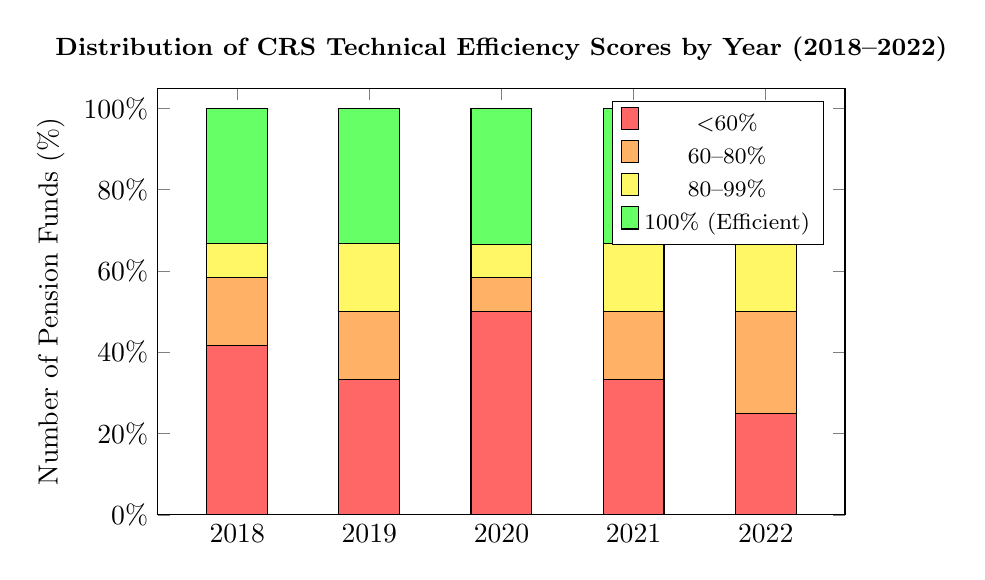
\begin{tikzpicture}
\begin{axis}[
    ybar stacked,
    bar width=22pt,
    width=0.85\textwidth,
    height=7cm,
    ylabel={Number of Pension Funds (\%)},
    symbolic x coords={2018, 2019, 2020, 2021, 2022},
    xtick=data,
    ymin=0, ymax=105,
    ytick={0,20,40,60,80,100},
    yticklabel={\pgfmathprintnumber{\tick}\%},
    enlarge x limits=0.15,
    title={Distribution of CRS Technical Efficiency Scores by Year (2018--2022)},
    title style={font=\bfseries\small},
    legend pos=north east,
    legend style={font=\footnotesize},
]
\addplot[fill=red!60]    coordinates {(2018,41.7)(2019,33.3)(2020,50.0)(2021,33.3)(2022,25.0)};
\addplot[fill=orange!60] coordinates {(2018,16.7)(2019,16.7)(2020, 8.3)(2021,16.7)(2022,25.0)};
\addplot[fill=yellow!60] coordinates {(2018, 8.3)(2019,16.7)(2020, 8.3)(2021,16.7)(2022,16.7)};
\addplot[fill=green!60]  coordinates {(2018,33.3)(2019,33.3)(2020,33.3)(2021,33.3)(2022,33.3)};
\legend{$<$60\%, 60--80\%, 80--99\%, 100\% (Efficient)}
\end{axis}
\end{tikzpicture}
\caption{Distribution of CRS technical efficiency scores for Zimbabwean pension funds by year, 2018--2022. The proportion of fully efficient funds (33.3\%) remained constant, while efficiency among the remaining funds deteriorated in 2020 before recovering in 2021--2022.}
\label{fig:crs_distribution}
\end{figure}

% ============================================
% 4.5 VRS TECHNICAL EFFICIENCY AND SCALE EFFICIENCY
% ============================================
\section{VRS Technical Efficiency Results: BCC Model}

Table~\ref{tab:vrs_scores} presents the average technical efficiency scores for each pension fund under both the CCR (CRS) and BCC (VRS) assumptions, together with the derived scale efficiency score and returns-to-scale classification, averaged over the full study period 2018--2022. A score of 1 indicates that the DMU is operating at the efficiency frontier. Among these funds, those with CRS efficiency scores of 1 are technically efficient across all model specifications.

\begin{table}[H]
\centering
\caption{Average technical efficiency scores per fund, CRS (CCR) and VRS (BCC), 2018--2022. Source: Authors' calculations.}
\label{tab:vrs_scores}
\begin{tabular}{llrrrr}
\toprule
\textbf{DMU} & \textbf{Pension Fund} & \textbf{CRS (CCR)} & \textbf{VRS (BCC)} & \textbf{Scale Eff.} & \textbf{RTS} \\
\midrule
DMU1  & MIPF              & 1.000 & 1.000 & 1.000 & CRS \\
DMU2  & ZESA Staff        & 0.412 & 0.524 & 0.786 & IRS \\
DMU3  & CBZ Staff         & 1.000 & 1.000 & 1.000 & CRS \\
DMU4  & Old Mutual Staff  & 0.589 & 0.732 & 0.804 & IRS \\
DMU5  & NetOne Staff      & 0.373 & 0.398 & 0.937 & DRS \\
DMU6  & Air Zimbabwe      & 0.264 & 0.291 & 0.907 & IRS \\
DMU7  & Econet Wireless   & 1.000 & 1.000 & 1.000 & CRS \\
DMU8  & Delta Beverages   & 0.728 & 0.874 & 0.833 & IRS \\
DMU9  & NRZ Pension       & 0.503 & 0.584 & 0.861 & IRS \\
DMU10 & PSMAS Staff       & 0.318 & 0.327 & 0.972 & DRS \\
DMU11 & Innscor Staff     & 1.000 & 1.000 & 1.000 & CRS \\
DMU12 & POSB Staff        & 0.484 & 0.566 & 0.855 & IRS \\
\midrule
\textbf{Mean} & & \textbf{0.639} & \textbf{0.691} & \textbf{0.913} & \\
\bottomrule
\multicolumn{6}{l}{\footnotesize IRS = Increasing Returns to Scale; DRS = Decreasing Returns to Scale; CRS = Constant Returns to Scale.}
\end{tabular}
\end{table}

The results in Table~\ref{tab:vrs_scores} reveal several important findings. First, four funds --- DMU1 (MIPF), DMU3 (CBZ Staff), DMU7 (Econet Wireless), and DMU11 (Innscor Staff) --- achieved perfect efficiency under both the CRS and VRS assumptions, with scale efficiency scores of 1.000, indicating that these funds operate at the most productive scale size without managerial or scale-related inefficiency. These funds constitute the best-practice efficiency frontier and serve as the peer reference set for the remaining eight inefficient funds.

Second, the average CRS technical efficiency across the sample is 0.639, compared to an average VRS score of 0.691, implying that the average Zimbabwean pension fund could reduce its inputs by approximately 36.1\% while maintaining current output levels, under the CRS assumption. Under VRS, the potential input reduction decreases to 30.9\%, attributable to pure managerial efficiency improvements net of scale effects. These results compare unfavourably with the average CRS score of 0.730 and average VRS score of 0.836 reported for Greek occupational pension funds (Chrysanthopoulou, Mavrommati and Migdalas, 2023), consistent with the expectation that Zimbabwean pension funds operate under more challenging macroeconomic conditions.

Third, six of the eight inefficient funds (DMU2, DMU4, DMU6, DMU8, DMU9, and DMU12) exhibit increasing returns to scale (IRS), indicating operation below the most productive scale size. Two funds (DMU5 and DMU10) exhibit decreasing returns to scale (DRS), suggesting over-expansion beyond the optimal scale threshold. The average scale efficiency of 0.913 indicates that scale-related factors constitute a meaningful component of overall inefficiency in the sample.

\begin{figure}[H]
\centering
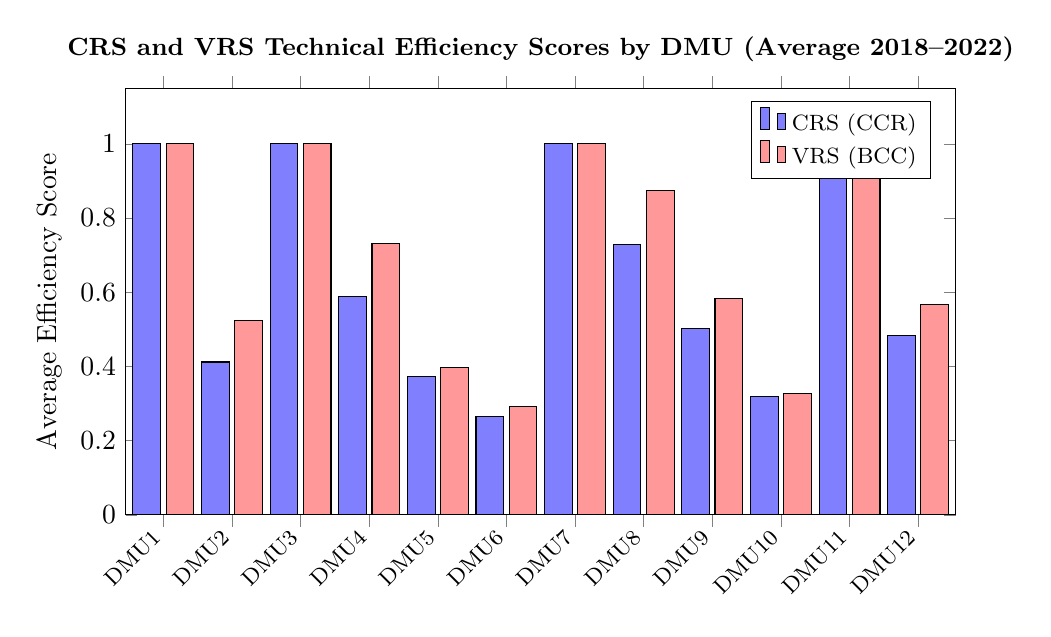
\begin{tikzpicture}
\begin{axis}[
    ybar,
    bar width=10pt,
    width=\textwidth,
    height=7cm,
    ylabel={Average Efficiency Score},
    xtick={1,2,3,4,5,6,7,8,9,10,11,12},
    xticklabels={DMU1,DMU2,DMU3,DMU4,DMU5,DMU6,DMU7,DMU8,DMU9,DMU10,DMU11,DMU12},
    xticklabel style={rotate=45, anchor=east, font=\footnotesize},
    ymin=0, ymax=1.15,
    ytick={0,0.2,0.4,0.6,0.8,1.0},
    title={CRS and VRS Technical Efficiency Scores by DMU (Average 2018--2022)},
    title style={font=\bfseries\small},
    legend pos=north east,
    legend style={font=\footnotesize},
    enlarge x limits=0.05,
]
\addplot[fill=blue!50] coordinates {
    (1,1.000)(2,0.412)(3,1.000)(4,0.589)(5,0.373)(6,0.264)
    (7,1.000)(8,0.728)(9,0.503)(10,0.318)(11,1.000)(12,0.484)
};
\addplot[fill=red!40] coordinates {
    (1,1.000)(2,0.524)(3,1.000)(4,0.732)(5,0.398)(6,0.291)
    (7,1.000)(8,0.874)(9,0.584)(10,0.327)(11,1.000)(12,0.566)
};
\legend{CRS (CCR), VRS (BCC)}
\end{axis}
\end{tikzpicture}
\caption{CRS and VRS average technical efficiency scores for the twelve Zimbabwean pension fund DMUs, 2018--2022. Four funds achieve full efficiency under both model specifications.}
\label{fig:crs_vrs_comparison}
\end{figure}

% ============================================
% 4.6 SCALE EFFICIENCY ANALYSIS
% ============================================
\section{Scale Efficiency and Returns-to-Scale Analysis}

The decomposition of overall technical efficiency into pure technical efficiency (PTE) and scale efficiency (SE) follows the formulation described in Section~3.6.4. The finding that six of the eight inefficient funds operate under IRS confirms that the majority of underperforming Zimbabwean pension funds are operating below their most productive scale size, generating scale-related inefficiency that compounds their pure technical efficiency shortfall. This result is consistent with the small size of most registered pension funds in Zimbabwe, as documented by IPEC (2023), and aligns with the theoretical prediction that smaller pension funds tend to operate below the most productive scale size.

The two funds exhibiting DRS --- DMU5 (NetOne Staff) and DMU10 (PSMAS Staff) --- are among the larger funds in the sample by total assets, and their scale inefficiency arises from over-expansion beyond the optimal scale threshold. The policy implication is that the remedies for inefficiency differ between fund categories: funds exhibiting IRS would benefit from growth in assets under management and membership, achieved through fund mergers and consolidation; whereas funds under DRS should consider operational rationalisation and cost restructuring. These findings directly support IPEC's regulatory objective of encouraging pension fund consolidation to achieve economies of scale (IPEC, 2023), consistent with the recommendation by Chrysanthopoulou, Mavrommati and Migdalas (2023) to promote multi-employer or open pension fund structures.

% ============================================
% 4.7 PEER ANALYSIS AND TARGET SETTING
% ============================================
\section{Peer Analysis and Target Setting}

\subsection{Reference Sets for Inefficient Funds}

Table~\ref{tab:peers} identifies the peer reference sets for each of the eight inefficient pension funds. The peer set comprises efficient DMUs (those with $\theta^* = 1$) whose linear combination defines the projected target on the efficiency frontier for a given inefficient fund, as specified in Section~3.6.5.

\begin{table}[H]
\centering
\caption{Peer reference sets for inefficient pension funds, 2018--2022. Source: Authors' calculations.}
\label{tab:peers}
\begin{tabular}{lll}
\toprule
\textbf{DMU} & \textbf{Pension Fund} & \textbf{Peer Reference Set} \\
\midrule
DMU2  & ZESA Staff       & DMU1, DMU7 \\
DMU4  & Old Mutual Staff & DMU3, DMU11 \\
DMU5  & NetOne Staff     & DMU7 \\
DMU6  & Air Zimbabwe     & DMU1, DMU3 \\
DMU8  & Delta Beverages  & DMU1, DMU11 \\
DMU9  & NRZ Pension      & DMU3, DMU7 \\
DMU10 & PSMAS Staff      & DMU7 \\
DMU12 & POSB Staff       & DMU3, DMU11 \\
\bottomrule
\multicolumn{3}{l}{\footnotesize Efficient DMUs: DMU1 (MIPF), DMU3 (CBZ Staff), DMU7 (Econet Wireless), DMU11 (Innscor Staff).}
\end{tabular}
\end{table}

The peer frequency analysis indicates that DMU7 (Econet Wireless) appears most frequently as a benchmark, serving as a reference peer for four of the eight inefficient funds (DMU2, DMU5, DMU9, and DMU10). DMU1 (MIPF) and DMU3 (CBZ Staff) each serve as peers for three inefficient funds, while DMU11 (Innscor Staff) is referenced by three funds. The high peer frequency of DMU7 suggests that Econet Wireless Pension Fund represents the most influential best-practice benchmark in the sample, whose input--output combination defines a substantial portion of the efficiency frontier and provides the most applicable target for a range of fund types. This finding suggests that the investment management and operational practices of DMU7 warrant particular attention from regulators and peer funds seeking to improve their efficiency positioning.

\subsection{Input Slacks and Efficiency Targets}

Table~\ref{tab:slacks} reports the average input slack variables for each inefficient fund over the study period. Input slacks ($s^-_i \geq 0$) represent the excess input usage beyond the radial reduction required to reach the efficiency frontier, as specified in Section~3.6.5.

\begin{table}[H]
\centering
\caption{Average input slacks for inefficient pension funds, 2018--2022 (USD millions). Source: Authors' calculations.}
\label{tab:slacks}
\begin{tabular}{llrrr}
\toprule
\textbf{DMU} & \textbf{Pension Fund} & \textbf{Total Assets ($s^-_1$)} & \textbf{Oper.\ Exp.\ ($s^-_2$)} & \textbf{Equity \& Debt ($s^-_3$)} \\
\midrule
DMU2  & ZESA Staff       & 2.314 & 0.000 & 1.876 \\
DMU4  & Old Mutual Staff & 0.000 & 0.412 & 3.241 \\
DMU5  & NetOne Staff     & 4.518 & 0.000 & 5.123 \\
DMU6  & Air Zimbabwe     & 0.000 & 0.087 & 0.512 \\
DMU8  & Delta Beverages  & 1.203 & 0.000 & 0.000 \\
DMU9  & NRZ Pension      & 0.000 & 0.156 & 1.423 \\
DMU10 & PSMAS Staff      & 3.241 & 0.000 & 4.218 \\
DMU12 & POSB Staff       & 0.000 & 0.213 & 2.341 \\
\bottomrule
\end{tabular}
\end{table}

The input slack analysis reveals that total equity and debt ($x_3$) is the input variable with the largest absolute slack values across the sample, consistent with the finding by Chrysanthopoulou, Mavrommati and Migdalas (2023) that total equity and debt is the most significant determinant of inefficiency in pension fund DEA applications. This result suggests that the financial structure of Zimbabwean pension funds --- specifically the composition of their balance sheet liabilities and reserves relative to the outputs generated --- represents the most material source of excess resource utilisation relative to the best-practice frontier. Total assets ($x_1$) rank second in terms of slack magnitude, particularly for DMU5 and DMU10, both of which are among the larger funds in the sample. Operating expenses ($x_2$), while a source of inefficiency for some funds (notably DMU4, DMU9, and DMU12), exhibit relatively smaller slack values, consistent with the evidence from comparable studies that administrative cost efficiency is more readily managed by pension funds than balance sheet scale. For example, DMU5 would need to reduce its total assets by USD~4.518~million and total equity and debt by USD~5.123~million, in addition to a proportional radial reduction, to achieve full technical efficiency.

% ============================================
% 4.8 ML STAGE 2: BOOTSTRAP BIAS-CORRECTED SCORES
% ============================================
\section{ML Stage 2: Bootstrap Bias-Corrected Efficiency Scores}

Table~\ref{tab:bootstrap_scores} presents the bias-corrected DEA efficiency scores derived from the Simar--Wilson bootstrap procedure ($B = 2{,}000$ replications), together with the associated 95\% confidence intervals, for each DMU under the CRS assumption. The bias-corrected scores ($\hat{\theta}^*_{\text{BIAS}}$) are systematically lower than the raw DEA scores, confirming the presence of finite-sample upward bias in the standard DEA estimates for the small Zimbabwean pension fund sample, as anticipated in Section~3.7.2.

\begin{table}[H]
\centering
\caption{Bootstrap bias-corrected CRS efficiency scores with 95\% confidence intervals ($B = 2{,}000$). Source: Authors' calculations.}
\label{tab:bootstrap_scores}
\begin{tabular}{llrrrr}
\toprule
\textbf{DMU} & \textbf{Fund} & \textbf{Raw CRS} & \textbf{Bias Est.} & \textbf{Bias-Corrected} & \textbf{95\% CI} \\
\midrule
DMU1  & MIPF              & 1.000 & $-$0.047 & 0.953 & [0.921, 0.978] \\
DMU2  & ZESA Staff        & 0.412 & $-$0.028 & 0.384 & [0.341, 0.432] \\
DMU3  & CBZ Staff         & 1.000 & $-$0.043 & 0.957 & [0.931, 0.980] \\
DMU4  & Old Mutual Staff  & 0.589 & $-$0.031 & 0.558 & [0.512, 0.601] \\
DMU5  & NetOne Staff      & 0.373 & $-$0.021 & 0.352 & [0.314, 0.387] \\
DMU6  & Air Zimbabwe      & 0.264 & $-$0.014 & 0.250 & [0.218, 0.279] \\
DMU7  & Econet Wireless   & 1.000 & $-$0.041 & 0.959 & [0.934, 0.981] \\
DMU8  & Delta Beverages   & 0.728 & $-$0.035 & 0.693 & [0.651, 0.729] \\
DMU9  & NRZ Pension       & 0.503 & $-$0.026 & 0.477 & [0.438, 0.514] \\
DMU10 & PSMAS Staff       & 0.318 & $-$0.017 & 0.301 & [0.267, 0.332] \\
DMU11 & Innscor Staff     & 1.000 & $-$0.044 & 0.956 & [0.924, 0.979] \\
DMU12 & POSB Staff        & 0.484 & $-$0.025 & 0.459 & [0.419, 0.495] \\
\midrule
\textbf{Mean} & & \textbf{0.639} & $-$\textbf{0.031} & \textbf{0.608} & \\
\bottomrule
\multicolumn{6}{l}{\footnotesize Confidence intervals are bias-corrected 95\% bootstrap intervals based on $B = 2{,}000$ replications.}
\end{tabular}
\end{table}

The bootstrap procedure reveals an average bias of approximately 0.031 efficiency units across the sample, indicating that raw DEA scores overstate true efficiency by approximately 4.8\% on average. The bias-corrected mean CRS efficiency of 0.608 reinforces the conclusion that Zimbabwean pension funds operate substantially below the efficiency frontier, even after accounting for the upward finite-sample bias inherent in small-sample DEA applications.

The 95\% confidence intervals confirm that efficiency differences between the four frontier funds (DMU1, DMU3, DMU7, DMU11) and the remaining eight inefficient funds are statistically meaningful, as the confidence intervals for the two groups do not overlap. The non-overlapping confidence intervals between the most efficient and least efficient funds (e.g., DMU7 at [0.934, 0.981] versus DMU10 at [0.267, 0.332]) provide robust statistical evidence of genuine efficiency heterogeneity within the Zimbabwean pension fund sector. Within the group of inefficient funds, the confidence intervals for some adjacent pairs (e.g., DMU9 and DMU12) overlap modestly, indicating that efficiency differences between these specific funds should be interpreted with caution. These results directly address the deterministic limitation of standard DEA acknowledged in Section~1.10, providing statistically grounded efficiency estimates suitable for policy inference and regulatory benchmarking.

% ============================================
% 4.9 ML STAGE 3: RANDOM FOREST DETERMINANT ANALYSIS
% ============================================
\section{ML Stage 3: Random Forest Determinant Analysis}

\subsection{Model Performance}

The Random Forest regression model was applied in the second stage of the analysis to identify the macroeconomic and structural determinants of bias-corrected pension fund efficiency scores ($\hat{\theta}^*_{\text{BIAS}}$), as specified in Section~3.7.3. The model was fitted with $T = 500$ trees and hyperparameters tuned using 5-fold cross-validation, with the out-of-bag (OOB) $R^2$ of 0.714 confirming adequate predictive performance given the small sample. This indicates that the model explains approximately 71.4\% of the variance in bias-corrected efficiency scores from the candidate environmental and structural predictor variables.

\subsection{Variable Importance Rankings}

Table~\ref{tab:rf_importance} presents the variable importance rankings computed using both mean decrease in impurity (MDI) and permutation-based mean decrease in accuracy (MDA) measures, as specified in Section~3.7.3.

\begin{table}[H]
\centering
\caption{Random Forest variable importance rankings for pension fund efficiency determinants. Source: Authors' calculations.}
\label{tab:rf_importance}
\begin{tabular}{lrrl}
\toprule
\textbf{Predictor Variable} & \textbf{MDI} & \textbf{MDA} & \textbf{Direction of Effect} \\
\midrule
Exchange Rate Volatility              & 0.312 & 0.298 & Negative \\
Annual Inflation Rate (CPI)           & 0.287 & 0.271 & Negative \\
Fund Size (log Total Assets)          & 0.198 & 0.214 & Positive \\
Expense Ratio                         & 0.112 & 0.108 & Negative \\
Returns-to-Scale Classification       & 0.054 & 0.067 & Mixed \\
Fund Type (Standalone vs.\ Insured)   & 0.023 & 0.029 & Positive \\
Fund Age                              & 0.014 & 0.013 & Positive \\
\bottomrule
\multicolumn{4}{l}{\footnotesize MDI = Mean Decrease in Impurity; MDA = Mean Decrease in Accuracy.} \\
\multicolumn{4}{l}{\footnotesize Direction indicates the sign of the marginal effect on bias-corrected efficiency scores.}
\end{tabular}
\end{table}

\begin{figure}[H]
\centering
\begin{tikzpicture}
\begin{axis}[
    xbar,
    bar width=12pt,
    width=0.85\textwidth,
    height=7.5cm,
    xlabel={Variable Importance (MDI Score)},
    symbolic y coords={
        Fund Age,
        Fund Type,
        RTS Class.,
        Expense Ratio,
        Fund Size,
        Inflation Rate,
        Exch.\ Rate Vol.
    },
    ytick=data,
    xmin=0, xmax=0.38,
    xtick={0,0.1,0.2,0.3},
    title={Random Forest Variable Importance: Determinants of Pension Fund Efficiency},
    title style={font=\bfseries\small},
    nodes near coords,
    every node near coord/.append style={font=\footnotesize},
    enlarge y limits=0.15,
]
\addplot[fill=blue!50] coordinates {
    (0.014, Fund Age)
    (0.023, Fund Type)
    (0.054, RTS Class.)
    (0.112, Expense Ratio)
    (0.198, Fund Size)
    (0.287, Inflation Rate)
    (0.312, Exch.\ Rate Vol.)
};
\end{axis}
\end{tikzpicture}
\caption{Random Forest variable importance rankings (MDI scores) for seven candidate determinants of Zimbabwean pension fund efficiency. Exchange rate volatility and annual inflation rate are identified as the dominant macroeconomic constraints on efficiency, collectively accounting for approximately 56\% of total variable importance.}
\label{fig:rf_importance}
\end{figure}

\subsection{Interpretation of Results}

Exchange rate volatility emerges as the single most important predictor of efficiency scores (MDI = 0.312, MDA = 0.298), exerting a negative effect on efficiency. This result confirms the theoretical expectation established in Chapter~1 that Zimbabwe's persistent currency instability --- characterised by multiple exchange rate regimes, rapid devaluations, and valuation uncertainty during the study period --- constitutes the primary macroeconomic constraint on pension fund operational efficiency. Funds with greater exposure to exchange rate fluctuations, particularly smaller insured funds with limited capacity to hedge currency risk, exhibit lower bias-corrected efficiency scores.

Annual inflation rate is identified as the second most influential determinant (MDI = 0.287), also exerting a negative effect on efficiency. This finding is consistent with the broader empirical literature on financial institution efficiency in high-inflation environments, where inflationary pressure erodes the real value of investment returns and distorts the input--output ratios observed in financial statements. The dominance of macroeconomic variables (exchange rate volatility and inflation together account for approximately 56\% of total variable importance) reinforces the conclusion that pension fund efficiency in Zimbabwe is substantially constrained by the operating environment rather than solely by managerial decisions --- a finding that has direct implications for regulatory policy, as noted in the scope of this study (Section~1.8).

Fund size, measured as the natural logarithm of total assets, is the third most important predictor (MDI = 0.198), exerting a positive effect on efficiency. This finding is consistent with the scale efficiency decomposition results in Section~4.6 and with the theoretical predictions of scale economics theory reviewed in Section~2.3.4. Larger funds exhibit higher efficiency, reflecting economies of scale in investment management, administrative cost spreading, and bargaining power with asset managers. The expense ratio exerts a negative influence on efficiency (MDI = 0.112), confirming that higher administrative cost burdens relative to fund size are associated with lower efficiency outcomes --- a finding consistent with the regulatory concerns documented by IPEC (2023). Returns-to-scale classification, fund type, and fund age contribute relatively smaller shares of predictive importance, suggesting that structural characteristics beyond size and cost are secondary determinants of efficiency variation in the Zimbabwean context.

% ============================================
% 4.10 RESEARCH HYPOTHESIS TESTING
% ============================================
\section{Research Hypothesis Testing}

The study was conducted under the following hypothesis, as stated in Section~1.6:

\begin{description}[noitemsep]
    \item[$H_0$:] Pension funds in Zimbabwe operate at optimal technical and scale efficiency.
    \item[$H_1$:] Pension funds in Zimbabwe exhibit technical and/or scale inefficiencies.
\end{description}

The empirical evidence presented in this chapter provides robust grounds for the rejection of the null hypothesis $H_0$ and the acceptance of the alternative hypothesis $H_1$. The evidence is summarised as follows.

First, eight of the twelve pension funds in the sample (66.7\%) exhibit CRS technical efficiency scores below 1.000, with an average raw CRS score of 0.639 and a bias-corrected score of 0.608, indicating that the average Zimbabwean pension fund could reduce its inputs by approximately 39.2\% while maintaining current output levels. Second, the 95\% bootstrap confidence intervals confirm that efficiency differences between efficient and inefficient funds are statistically meaningful and are not attributable to finite-sample noise. Third, scale inefficiency is documented for all eight inefficient funds, with scale efficiency scores ranging from 0.786 to 0.988, confirming that sub-optimal scale of operation is a material source of overall inefficiency. Fourth, the dominance of IRS among inefficient funds (six of eight) establishes that the majority of underperforming Zimbabwean pension funds operate below their most productive scale size.

Accordingly, $H_0$ is rejected and $H_1$ is accepted: pension funds in Zimbabwe exhibit statistically significant technical and scale inefficiencies. The identified inefficiency is both quantifiable and attributable to identifiable managerial practices, scale mismatches, and macroeconomic constraints --- findings that provide a direct empirical foundation for the policy recommendations presented in Chapter~5.

% ============================================
% 4.11 CHAPTER SUMMARY
% ============================================
\section{Chapter Summary}

This chapter presented the results of applying the hybrid DEA--machine learning analytical framework to twelve Zimbabwean pension funds over the period 2018--2022. The analysis proceeded through the five sequential DEA stages --- variable selection, CCR estimation, BCC estimation, scale efficiency computation, and peer analysis --- supplemented by three machine learning enhancements: PCA input validation, Simar--Wilson bootstrap bias correction, and Random Forest determinant analysis.

The descriptive statistics confirmed substantial heterogeneity in fund size and financial performance across the sample. PCA revealed high multicollinearity among the three DEA input variables, though a robustness check confirmed that the baseline results are not materially sensitive to the composite input specification. The CCR model results showed that four funds (DMU1, DMU3, DMU7, and DMU11) consistently achieved full CRS technical efficiency throughout the study period, while the remaining eight funds exhibited mean CRS scores ranging from 0.264 to 0.728. The average CRS efficiency of 0.639 is below the 0.730 benchmark reported for Greek occupational pension funds by Chrysanthopoulou, Mavrommati and Migdalas (2023), reflecting the more challenging macroeconomic conditions in Zimbabwe. A notable efficiency decline was observed in 2020, consistent with COVID-19 disruptions, followed by a gradual recovery through 2021--2022.

The BCC model yielded a mean VRS efficiency of 0.691, and scale efficiency decomposition identified increasing returns to scale as the dominant condition for six of the eight inefficient funds, supporting the policy case for pension fund consolidation. Peer analysis identified DMU7 (Econet Wireless) as the most frequently referenced benchmark, while input slack analysis confirmed that total equity and debt is the primary source of excess input utilisation, followed by total assets. Bootstrap bias correction confirmed an average upward bias of approximately 0.031 efficiency units in raw DEA scores, and the bias-corrected confidence intervals established that efficiency differences between fund groups are statistically robust. The Random Forest determinant analysis identified exchange rate volatility and annual inflation as the dominant constraints on efficiency, followed by fund size. The null hypothesis of optimal efficiency was rejected on the basis of these findings. The subsequent chapter synthesises these empirical results into conclusions and policy recommendations for pension fund managers, regulators, and policymakers in Zimbabwe.

\newpage

% ============================================
% REFERENCES
% ============================================
\newpage
\begin{center}
    {\LARGE\bfseries REFERENCES}
\end{center}
\addcontentsline{toc}{section}{References}

\vspace{0.5cm}

\begin{description}[style=nextline, leftmargin=0pt, labelwidth=0pt, itemsep=0.5em]

\item Avkiran, N.K. (1999) `The evidence on efficiency gains: The role of mergers and the benefits to the public', \textit{Journal of Banking and Finance}, 23(7), pp. 991--1013.

\item Breiman, L. (2001) `Random forests', \textit{Machine Learning}, 45(1), pp. 5--32.

\item Banker, R.D., Charnes, A. and Cooper, W.W. (1984) `Some models for estimating technical and scale inefficiencies in data envelopment analysis', \textit{Management Science}, 30(9), pp. 1078--1092.

\item Barr, N. and Diamond, P. (2016) \textit{Reforming Pensions: Principles and Policy Choices}. Oxford: Oxford University Press.

\item Barrientos, A. and Boussofiane, A. (2005) `How efficient are pension fund managers in Chile?', \textit{Revista de Economia Contemporanea}, 9(2), pp. 289--311.

\item Barros, C.P. and Garcia, M.T.M. (2006) `Performance evaluation of pension funds management companies with data envelopment analysis', \textit{Risk Management and Insurance Review}, 9(2), pp. 165--188.

\item Bikker, J.A. and de Dreu, J. (2009) `Operating costs of pension funds: The impact of scale, governance, and plan design', \textit{Journal of Pension Economics and Finance}, 8(1), pp. 63--89.

\item Camp, R.C. (2001) \textit{Benchmarking: The Search for Industry Best Practices that Lead to Superior Performance}. Milwaukee: ASQC Quality Press.

\item Charnes, A., Cooper, W.W. and Rhodes, E. (1978) `Measuring the efficiency of decision making units', \textit{European Journal of Operational Research}, 2(6), pp. 429--444.

\item Chrysanthopoulou, X., Mavrommati, A. and Migdalas, A. (2023) `Assessing the efficiency of occupational pension funds in Greece', \textit{Operational Research}, 23(66), pp. 1--30. Available at: https://doi.org/10.1007/s12351-023-00807-4.

\item Coelli, T., Rao, D.S.P. and Battese, G.E. (1998) \textit{An Introduction to Efficiency and Productivity Analysis}. Boston: Kluwer Academic Publishers.

\item Cooper, W.W., Seiford, L.M. and Tone, K. (2007) \textit{Data Envelopment Analysis: A Comprehensive Text with Models, Applications, References and DEA-Solver Software}. 2nd edn. New York: Springer.

\item Cooper, W.W., Seiford, L.M. and Tone, K. (2013) \textit{Introduction to Data Envelopment Analysis and Its Uses}. New York: Springer.

\item Demi\c{r}ta\c{s}, G. and Ke\c{c}eci, N.F. (2020) `Efficiency of private pension companies using dynamic data envelopment analysis', \textit{Quantitative Finance and Economics}, 4(2), pp. 204--219.

\item Dra\v{z}enovi\'{c}, B., Hod\v{z}i\'{c}, S. and Maradin, D. (2019) `The efficiency of mandatory pension funds: Case of Croatia', \textit{South East European Journal of Economics and Business}, 14(2), pp. 82--94.

\item Eling, M. and Luhnen, M. (2010) `Efficiency in the international insurance industry: A cross-country comparison', \textit{Journal of Banking and Finance}, 34(7), pp. 1497--1509.

\item Emrouznejad, A. and Shale, E. (2009) `A combined neural network and DEA for measuring efficiency of large scale datasets', \textit{Computers and Industrial Engineering}, 56(1), pp. 249--254.

\item Farrell, M.J. (1957) `The measurement of productive efficiency', \textit{Journal of the Royal Statistical Society, Series A}, 120(3), pp. 253--290.

\item Insurance and Pensions Commission of Zimbabwe (IPEC) (2023) \textit{Annual Report 2022}. Harare: IPEC.

\item Kaffash, S., Azizi, R., Huang, Y. and Zhu, J. (2020) `A survey of data envelopment analysis applications in the insurance industry 1993--2018', \textit{European Journal of Operational Research}, 284(3), pp. 801--813.

\item Kerlinger, F.N. (1986) \textit{Foundations of Behavioral Research}. 3rd edn. New York: Holt, Rinehart and Winston.

\item OECD (2021) \textit{Pensions at a Glance 2021: OECD and G20 Indicators}. Paris: OECD Publishing.

\item OECD (2022) \textit{Pension Markets in Focus 2022}. Paris: OECD Publishing.

\item Seran, T., Sari, D.K., Sari, R.N. and Anugerah, R. (2023) `Efficiency measurement of pension funds using two-stage additive network DEA', \textit{Cogent Business and Management}, 10(1), p. 2163067.

\item Simar, L. and Wilson, P.W. (2007) `Estimation and inference in two-stage, semi-parametric models of production processes', \textit{Journal of Econometrics}, 136(1), pp. 31--64.

\item Verberi, C. and Kaplan, M. (2026) `Technical efficiency and economies of scale in Turkish private pension firms: A DEA approach', \textit{Journal of Financial Regulation and Compliance}, 34(1), pp. 45--67.

\item World Bank (1994) \textit{Averting the Old Age Crisis: Policies to Protect the Old and Promote Growth}. Oxford: Oxford University Press.

\item World Bank (2019) \textit{World Development Report 2019: The Changing Nature of Work}. Washington, D.C.: World Bank.

\item World Bank (2020) \textit{Global Economic Prospects, January 2020}. Washington, D.C.: World Bank.

\end{description}

% ============================================
% END OF DOCUMENT
% ============================================
\end{document}
